\documentclass{article}

\usepackage{fancyhdr}
\usepackage{extramarks}
\usepackage{amsmath}
\usepackage{amsthm}
\usepackage{amsfonts}
\usepackage{tikz}
\usepackage[plain]{algorithm}
\usepackage{algpseudocode}
\usepackage[]{mcode}
\usepackage{graphicx}
\usepackage{epstopdf}
\usepackage{siunitx}
\usepackage{xfrac}

\usetikzlibrary{automata,positioning}

%
% Basic Document Settings
%

\topmargin=-0.45in
\evensidemargin=0in
\oddsidemargin=0in
\textwidth=6.5in
\textheight=9.0in
\headsep=0.25in

\linespread{1.1}

\pagestyle{fancy}
\lhead{\hmwkAuthorName}
\chead{\hmwkClass\ (\hmwkClassInstructor\ \hmwkClassTime): \hmwkTitle}
\rhead{\firstxmark}
\lfoot{\lastxmark}
\cfoot{\thepage}

\renewcommand\headrulewidth{0.4pt}
\renewcommand\footrulewidth{0.4pt}

\setlength\parindent{0pt}

%
% Create Problem Sections
%

\newcommand{\enterProblemHeader}[1]{
    \nobreak\extramarks{}{Problem \arabic{#1} continued on next page\ldots}\nobreak{}
    \nobreak\extramarks{Problem \arabic{#1} (continued)}{Problem \arabic{#1} continued on next page\ldots}\nobreak{}
}

\newcommand{\exitProblemHeader}[1]{
    \nobreak\extramarks{Problem \arabic{#1} (continued)}{Problem \arabic{#1} continued on next page\ldots}\nobreak{}
    \stepcounter{#1}
    \nobreak\extramarks{Problem \arabic{#1}}{}\nobreak{}
}

\setcounter{secnumdepth}{0}
\newcounter{partCounter}
\newcounter{homeworkProblemCounter}
\setcounter{homeworkProblemCounter}{1}
\nobreak\extramarks{Problem \arabic{homeworkProblemCounter}}{}\nobreak{}

%
% Homework Problem Environment
%
% This environment takes an optional argument. When given, it will adjust the
% problem counter. This is useful for when the problems given for your
% assignment aren't sequential. See the last 3 problems of this template for an
% example.
%
\newenvironment{homeworkProblem}[1][-1]{
    \ifnum#1>0
        \setcounter{homeworkProblemCounter}{#1}
    \fi
    \section{Problem \arabic{homeworkProblemCounter}}
    \setcounter{partCounter}{1}
    \enterProblemHeader{homeworkProblemCounter}
}{
    \exitProblemHeader{homeworkProblemCounter}
}

%
% Homework Details
%   - Title
%   - Due date
%   - Class
%   - Section/Time
%   - Instructor
%   - Author
%

\newcommand{\hmwkTitle}{Tutorial\ 4}
\newcommand{\hmwkDueDate}{April 7, 2017}
\newcommand{\hmwkClass}{Digital Signal Processing}
\newcommand{\hmwkClassTime}{}
\newcommand{\hmwkClassInstructor}{Friso DeBoer}
\newcommand{\hmwkAuthorName}{S.Reynolds (262538)}

%
% Title Page
%

\title{
    \vspace{2in}
    \textmd{\textbf{\hmwkClass:\ \hmwkTitle}}\\
    \normalsize\vspace{0.1in}\small{Due\ on\ \hmwkDueDate\ at 3:00pm}\\
    \vspace{0.1in}\large{\textit{\hmwkClassInstructor\ \hmwkClassTime}}
    \vspace{3in}
}

\author{\textbf{\hmwkAuthorName}}
\date{}

\renewcommand{\part}[1]{\textbf{\large Part \Alph{partCounter}}\stepcounter{partCounter}\\}

%
% Various Helper Commands
%

% Useful for algorithms
\newcommand{\alg}[1]{\textsc{\bfseries \footnotesize #1}}

% For derivatives
\newcommand{\deriv}[1]{\frac{\mathrm{d}}{\mathrm{d}x} (#1)}

% For partial derivatives
\newcommand{\pderiv}[2]{\frac{\partial}{\partial #1} (#2)}

% Integral dx
\newcommand{\dx}{\mathrm{d}x}

% Alias for the Solution section header
\newcommand{\solution}{\textbf{\large Solution}}

% Probability commands: Expectation, Variance, Covariance, Bias
\newcommand{\E}{\mathrm{E}}
\newcommand{\Var}{\mathrm{Var}}
\newcommand{\Cov}{\mathrm{Cov}}
\newcommand{\Bias}{\mathrm{Bias}}

\graphicspath{{../Images/}}

\begin{document}

\maketitle

\pagebreak

\section{2.1 Frequency Response of the Three-Point Averager}

\subsection{Part A}

The three-point averager filter, $y[n]$, can be described by the following equation:
\begin{align}
	y[n] = \frac{1}{3} \cdot \sum_{k=0}^{2}x[n-k]
\end{align}

To find the frequency response function consider the input signal $x[n] = A \cdot e^{j \hat{\omega}n + \phi}$. If this signal is run through the filter shown in equation (1), then we get that:
\begin{align*}
	y[n] 	&= \frac{1}{3} \sum_{k=0}^{2} A \cdot e^{j \hat{\omega}k + \phi}\\
			&= \frac{1}{3} \cdot (A \cdot e^{j \hat{\omega}n + \phi} + A \cdot e^{j \hat{\omega}(n-1) + \phi} + A \cdot e^{j \hat{\omega}(n-2) + \phi})\\
			&= \frac{1}{3} \cdot A \cdot e^{j \hat{\omega}n + \phi} \cdot (1 + e^{-j \hat{\omega}} + e^{-2j \hat{\omega}})
\end{align*}

Hence, the output gives us the original signal input back, $A \cdot e^{j \hat{\omega}n + \phi}$, and we get the frequency response function $H(e^{j \hat{\omega}})$. The frequency response function is as follows:
\begin{align*}
	H(e^{j \hat{\omega}}) 	&= \frac{1}{3} \cdot (1 + e^{-j \hat{\omega}} + e^{-2j \hat{\omega}})\\
							&= \frac{1}{3} \cdot (e^{-j \hat{\omega}} + 1 + e^{j \hat{\omega}}) \cdot e^{j \hat{\omega}}\\
							&= \frac{1}{3} \cdot (\cos(j \hat{\omega}) - j \sin(j \hat{\omega}) + 1 + \cos(j \hat{\omega}) + j \sin(j \hat{\omega})) \cdot e^{j \hat{\omega}}\\
							&= \frac{1}{3} \cdot (2 \cos(j \hat{\omega}) + 1) \cdot e^{j \hat{\omega}}\\
							&= \frac{2 \cos(j \hat{\omega} + 1)}{3} \cdot e^{j \hat{\omega}}
\end{align*}

\subsection{Part B}

The above transfer function (frequency response function) was implemented in MATLAB using the following code:

\begin{lstlisting}
	%%%%%%%%% 2.1 Frequency Response of the Three-Point Averager %%%%%%%%%%%
	
	% Clear the workspace and any stored variables
	clear; clc;
	
	% Initialise parameters that will be used for the averager
	ww = linspace(-pi,pi,400);
	
	% Implementation of of the frequency response function
	% (This is the same as the transfer function - different noteation?)
	H = ( (2*cos(ww) + 1)/3 ).* exp(-j*ww);
	
	% Plot the Magnitude of the frequency response
	subplot(2,1,1)
	plot(ww,abs(H))
	xlabel('frequency (rad/sec)')
	ylabel('magnitude |H|')
	
	% Plot the Phase Angle Shift of the frequency response
	subplot(2,1,2)
	plot(ww,angle(H))
	xlabel('frequency (rad/sec)')
	ylabel('phase shift (rad)')
\end{lstlisting}

The Bode plot of the output can be seen in Figure 1.

\begin{figure}[h]
	\centering
	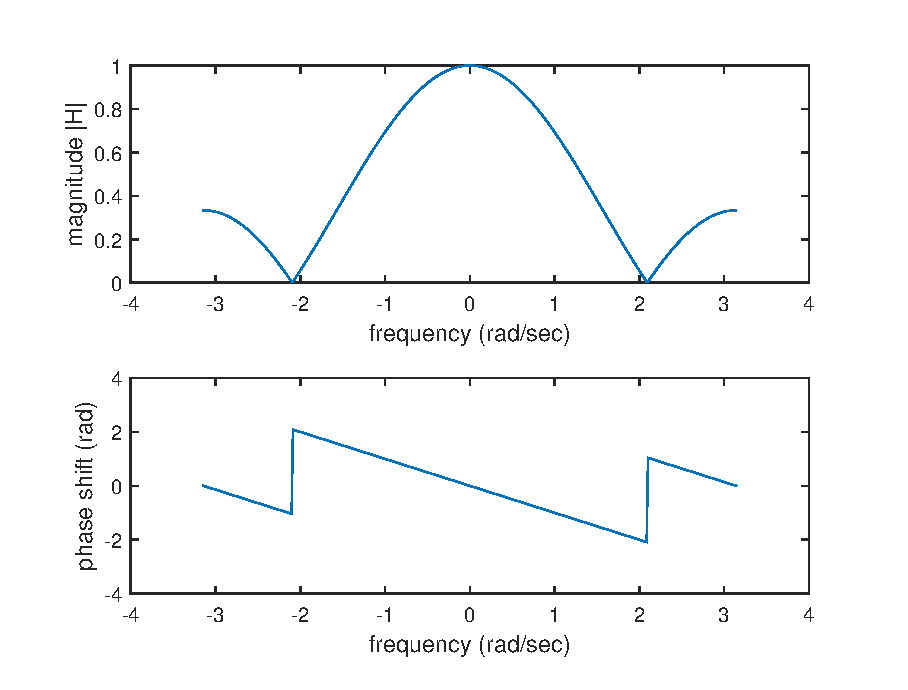
\includegraphics[scale=0.4]{fig1}
	\caption{A Bode plot of the frequency response function for the three point averager, implemented using the derived transfer function from Part A.}
\end{figure}

\begin{figure}[h]
		\centering
		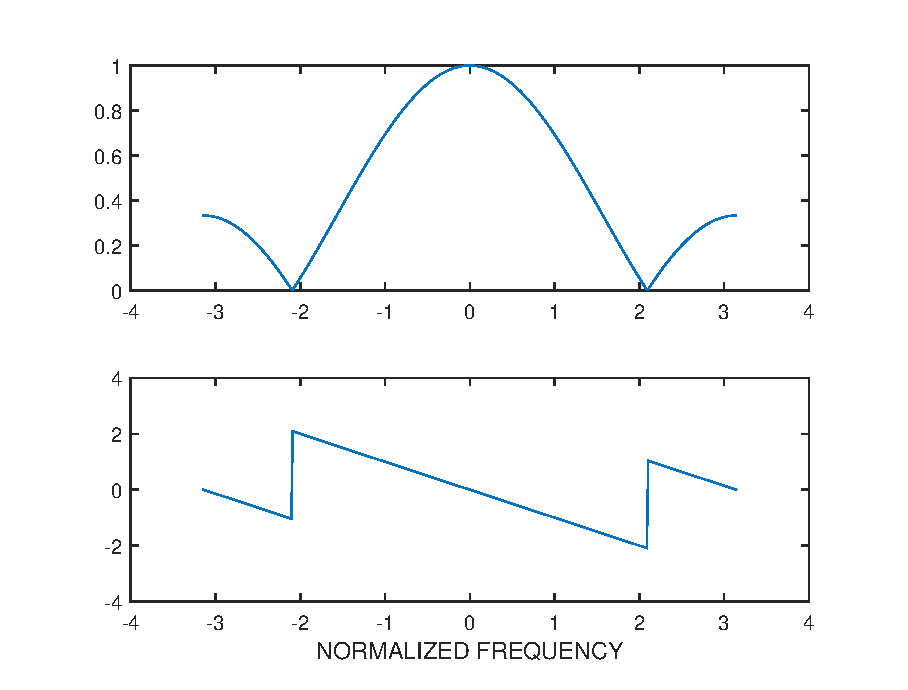
\includegraphics[scale=0.4]{fig2}
		\caption{A Bode plot of the frequency response function for the three point averager, implemented using the frequency response function in MATLAB from Part C.}
\end{figure}


There is no difference between the two plots shown in Figure 1 and Figure 2.

\subsection{Part C}

A Bode plot was created using the \verb|freqz()| MATLAB function. The Bode plot can be seen in Figure 2. The code that was used can be seen below:

\begin{lstlisting}
	%%%%%%%% 2.1 Fequency Response of the Three-Point Averager %%%%%%%%%%%
	
	% Clear the workspace and any stored variables
	clear; clc;
	
	% This script is provided by the tutorial assignment
	bb = 1/3*ones(1,3);
	ww = -pi:(pi/200):pi;
	H = freqz(bb,1,ww);
	subplot(2,1,1)
	plot(ww, abs(H))
	subplot(2,1,2)
	plot(ww, angle(H))
	xlabel('NORMALIZED FREQUENCY')
\end{lstlisting}

\section{3.2 First Difference Filter}

\subsection{Part A}
A cosine signal was generated using with amplitude, $A = 7$, a $\phi = \frac{\pi}{3}$, and $\hat{\omega} = 0.125 \pi$. The signal was passed through the first difference filter $y[n] = 5 \cdot x[n] - 5 \cdot x[n-1]$. The implementation of this in MATLAB can be seen in the following code:

\begin{lstlisting}
	%%%%%%%%%%%%%%%%% 3.2 First Difference Filter %%%%%%%%%%%%%%%%%%%
	% Code written by Shane Reynolds
	
	% Clear the workspace and any stored variables
	clear; clc;
	
	L = 50;
	
	% Create a vector which will be used to create samples
	nn = 0:(L-1);
	
	% Initialise the parameters used to define the input signal
	A = 7;
	ph = pi/3;
	ww = 0.125*pi;
	
	% Take discrete samples of the cosine
	xx = A*cos(ww*nn + ph);
	
	% Create the filter and the associated response to teh input signal
	bb = [5 -5];
	yy = firfilt(bb,xx);
	
	% Create plots to compare the inpust signal with the output signal
	subplot(2,1,1)
	plot(nn,xx)
	xlabel('sample number')
	
	subplot(2,1,2)
	plot(nn,yy(1:50))
	xlabel('sample number')
\end{lstlisting}

\subsection{Part B}
The plot shown in Figure 3 show the signal prior to filtering on the top plot and the signal after filtering on the bottom plot. The amplitude of the signals can be found from visual inspection. The amplitude of the input is 7 and the amplitude of the output is roughly 14. The phase is a little bit more difficult to find. By inspection, we see that the input signal seems to be shifted to the left by 3 sample points. Now, the following is true when determining phase shift for a discrete signal which has been shifted by $n_0$ sample points:
\begin{align*}
	x[n + n_0]  &= A \cdot \cos(\hat{\omega} \cdot (n - n_0))\\
				&= A \cdot \cos(\hat{\omega} \cdot n - \hat{\omega} \cdot n_0)
\end{align*}

\begin{figure}[H]
	\centering
	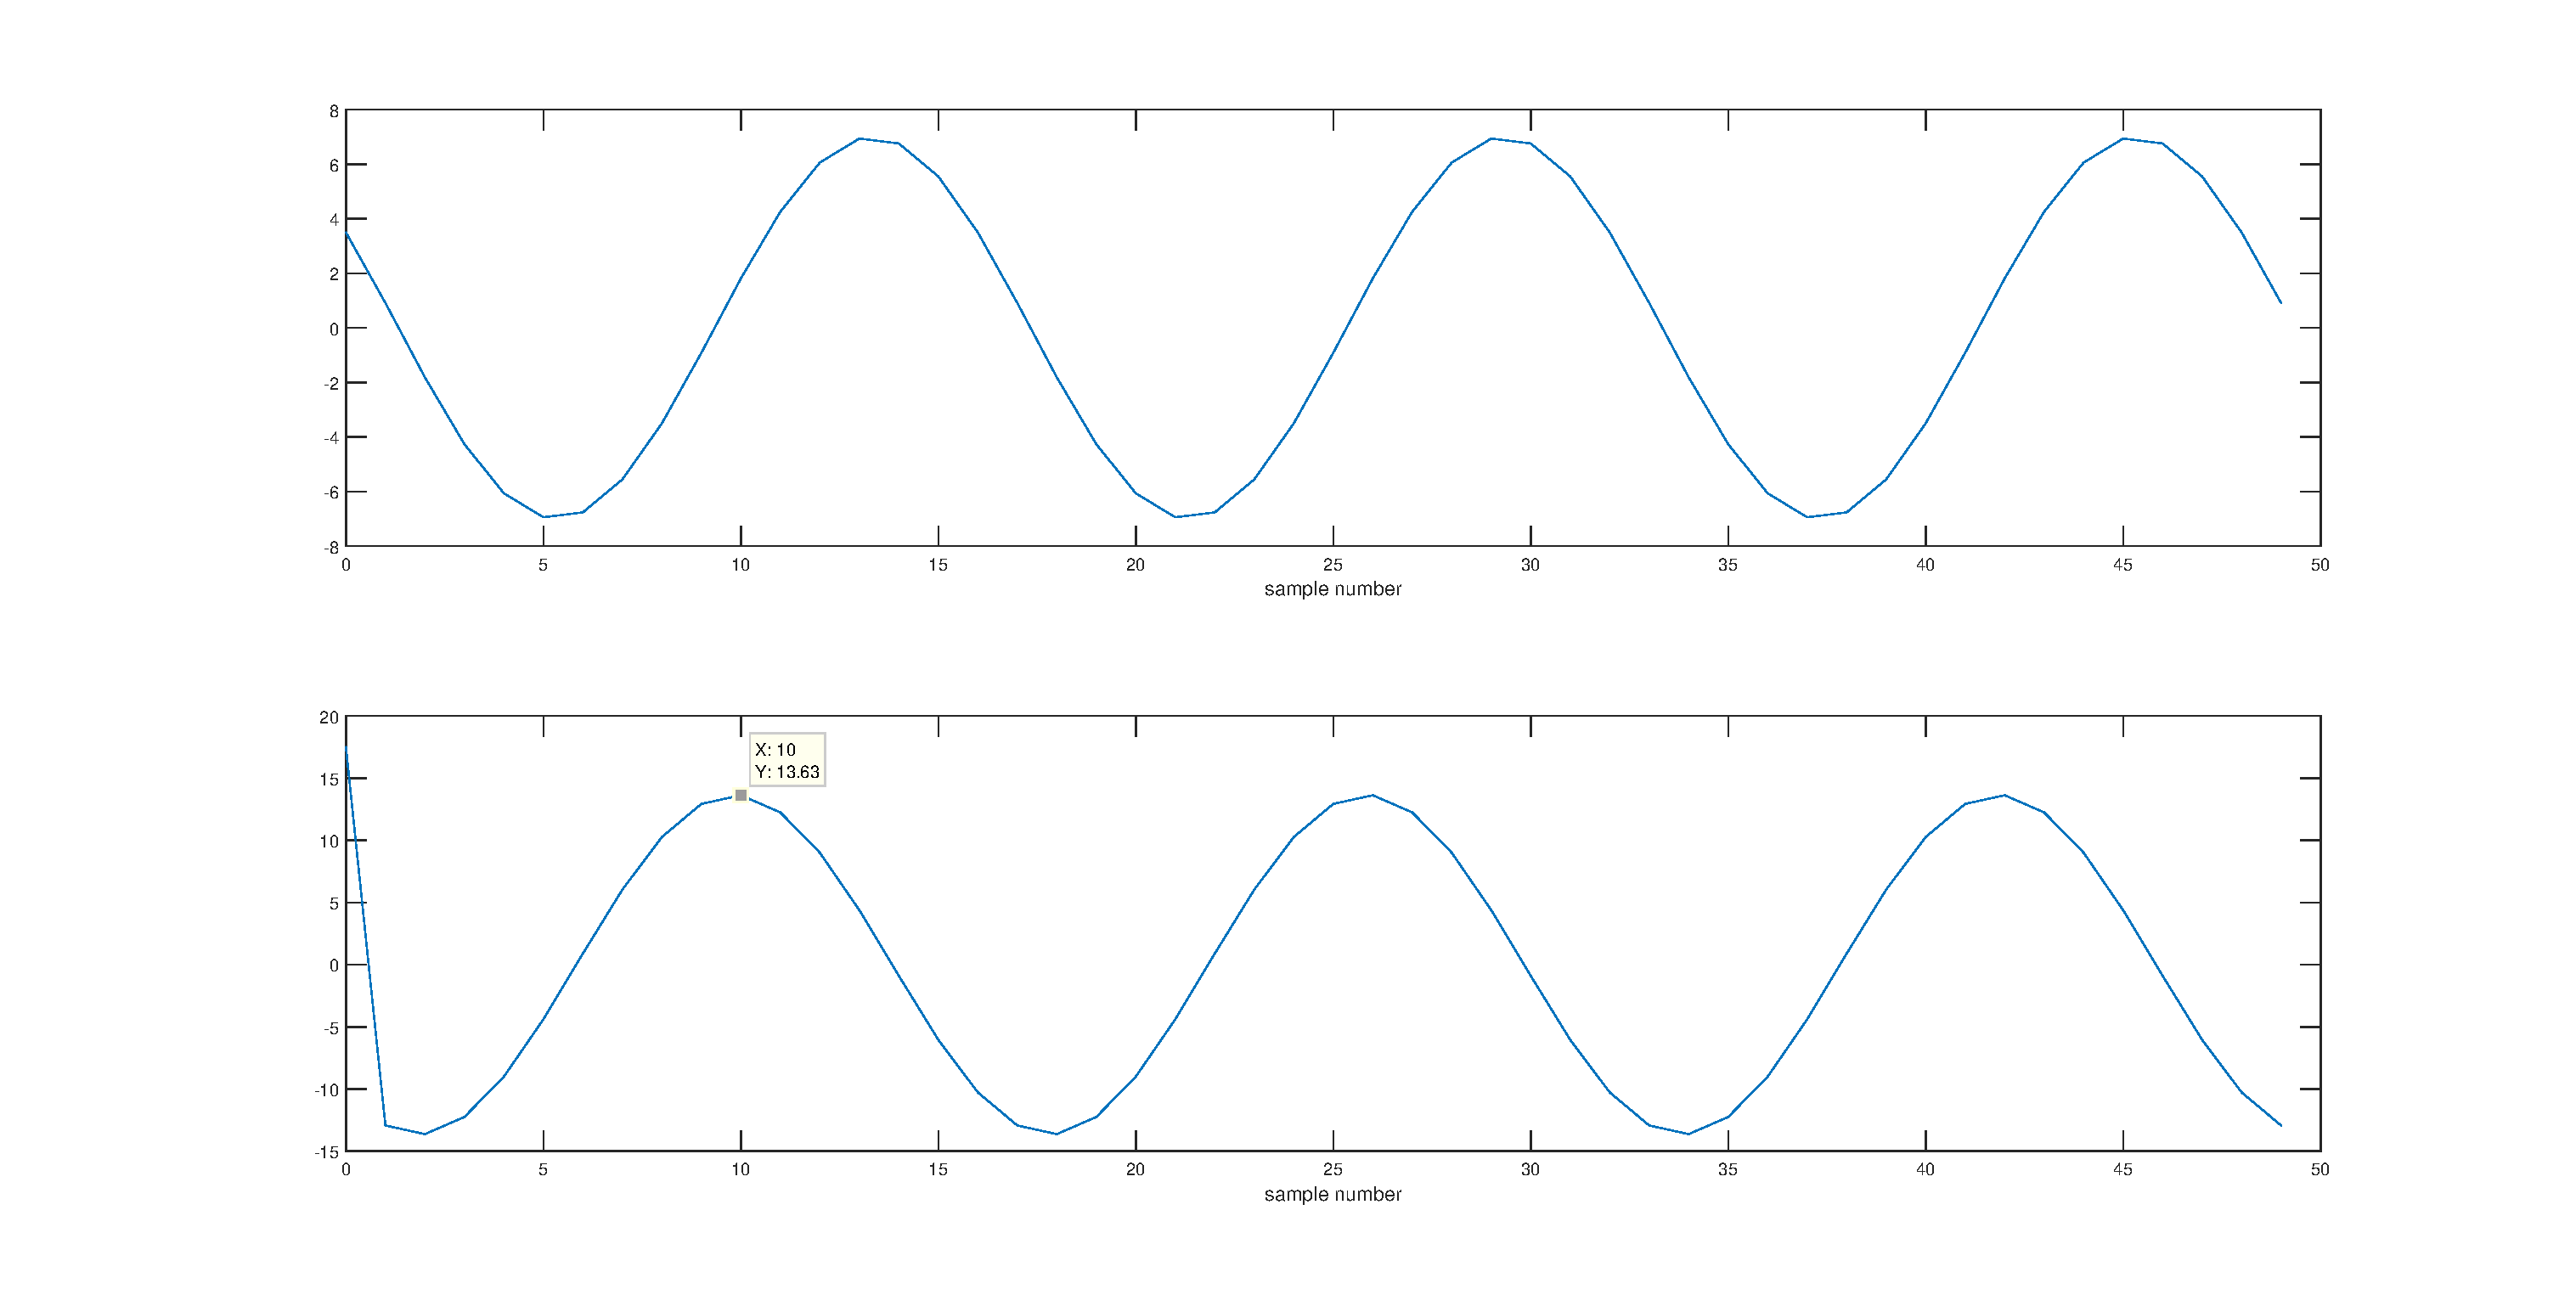
\includegraphics[scale = 0.3]{fig3}
	\caption{Time series plot of input signal and filtered signal, using a first difference filter}
\end{figure}

\subsection{Part C}
Hence, we see that the phase shift is given by $\hat{\omega} \cdot n_0$. In the case of the input signal, we see that the phase shift is roughly 3 sample points. This means that the phase shift is approximately $0.33 \pi$. The output phase shift is approximately 6.5 sample points which means the phase shift is approximately $0.8125 \pi$.

\subsection{Part D}
We note that the first sample of the output doesn't seem to appear correctly. This is due the nature of the filter through which the signal is passed. The filter requires the present value and a past value to provide the output at the point $n = 0$ we see that there doesn't exist a point at $n=-1$, and so the calculation performed by the MATLAB implementation is incorrect. In fact, this point should probably be left out of the output signal to avoid error being propagated through further processes.

\subsection{Part F}
The filter has a gain given by:
\begin{align*}
	\frac{|y[n]|}{|x[n]|} = \frac{14}{7} = 2
\end{align*}

Further, the phase shift of the filter can be found as:
\begin{align*}
	\angle \bigg(\sfrac{y[n]}{x[n]}\bigg) = 0.8125 \pi - 0.33 \pi = 0.4825 \pi
\end{align*}

\subsection{Part G}
Mathematically, we can derive the amplitude gain and phase shift of the filter. If we consider the input signal $x[n] = A \cdot e^{j \hat{\omega}n - \phi}$, and we input this to the filter, we get:
\begin{align*}
	y[n] 	&= 5 \cdot A \cdot e^{j \hat{\omega}n - \phi} - 5 \cdot A \cdot e^{j \hat{\omega}(n-1) - \phi}\\
			&= A \cdot e^{j \hat{\omega}n - \phi} \cdot 5 \cdot (1 - e^{-j \hat{\omega}})
\end{align*}

Hence, we find that:
\begin{align*}
	\frac{y[n]}{x[n]} 	&= 5 \cdot (1 - e^{-j \hat{\omega}})\\
						&= 5 - 5 \cdot \cos(j \hat{\omega}) + j \cdot \sin(j \hat{\omega})
\end{align*}

The frequency response function is given by:
\begin{align*}
	H(\hat{\omega}) = 5 - 5 \cdot \cos(j \hat{\omega}) + j \cdot \sin(j \hat{\omega})
\end{align*}

Given that the discrete time frequency, $\hat{\omega}$, is $0.125 \pi$, we see that the magnitude of the response is given by:
\begin{align*}
	|H(0.125 \pi)| 	&= |5 - 5 \cdot \cos(0.125 \pi) + j \cdot \sin(0.125 \pi)|\\
					&= \sqrt{(5 - 5 \cdot \cos(0.125 \pi)^2 + (\sin(0.125 \pi))^2)}\\
					&= 1.95
\end{align*}

The phase shift is given by:
\begin{align*}
	\angle H(0.125 \pi) &= \tan^{-1}\bigg(\frac{\sin(0.125 \pi)}{5 - 5 \cdot \cos(0.125 \pi)}\bigg)\\
						&= 1.37 \ \si{\radian}
\end{align*}

We note that there is a calculation error (or estimation error in the phase shift) - the two values don't match up.

\section{3.3 Linearity of the Filter}

\subsection{Part A}

A code was implemented which scales the first input by a factor of 2. The code implementation can be seen below:
\begin{lstlisting}
	%%%%%%%%%%%%% 3.3 Linearity of the Filter %%%%%%%%%%%%%%%%%%
	
	% Clear the worksapce and any stored variables
	clear; clc;
	
	L = 50;
	
	% Create a vector which will be used to create samples
	nn = 0:(L-1);
	
	% Initialise the parameters used to define the input signal
	A = 7;
	ph = pi/3;
	ww = 0.125*pi;
	
	% Take discrete samples of the cosine
	xx = A*cos(ww*nn + ph);
	
	% Create a linearly scaled version of xx
	xa = 2*xx;
	
	% Create the filter and the associated response to teh input signal
	bb = [5 -5];
	ya = firfilt(bb,xa);
	
	% Create plots to compare the inpust signal with the output signal
	subplot(2,1,1)
	plot(nn,xa)
	
	subplot(2,1,2)
	plot(nn,ya(1:50))
\end{lstlisting}

A plot of the time series plots can be seen in Figure 4. By inspection we can see that the input signal has an amplitude of 14 and a phase shift of approximately $0.33 \pi$. The output signal has an amplitude of 28 and a phase shift of $0.8125 \pi$. We note that scaling the input only scales the amplitude of the frequency response function by the same scalar amount.

\begin{figure}[H]
	\centering
	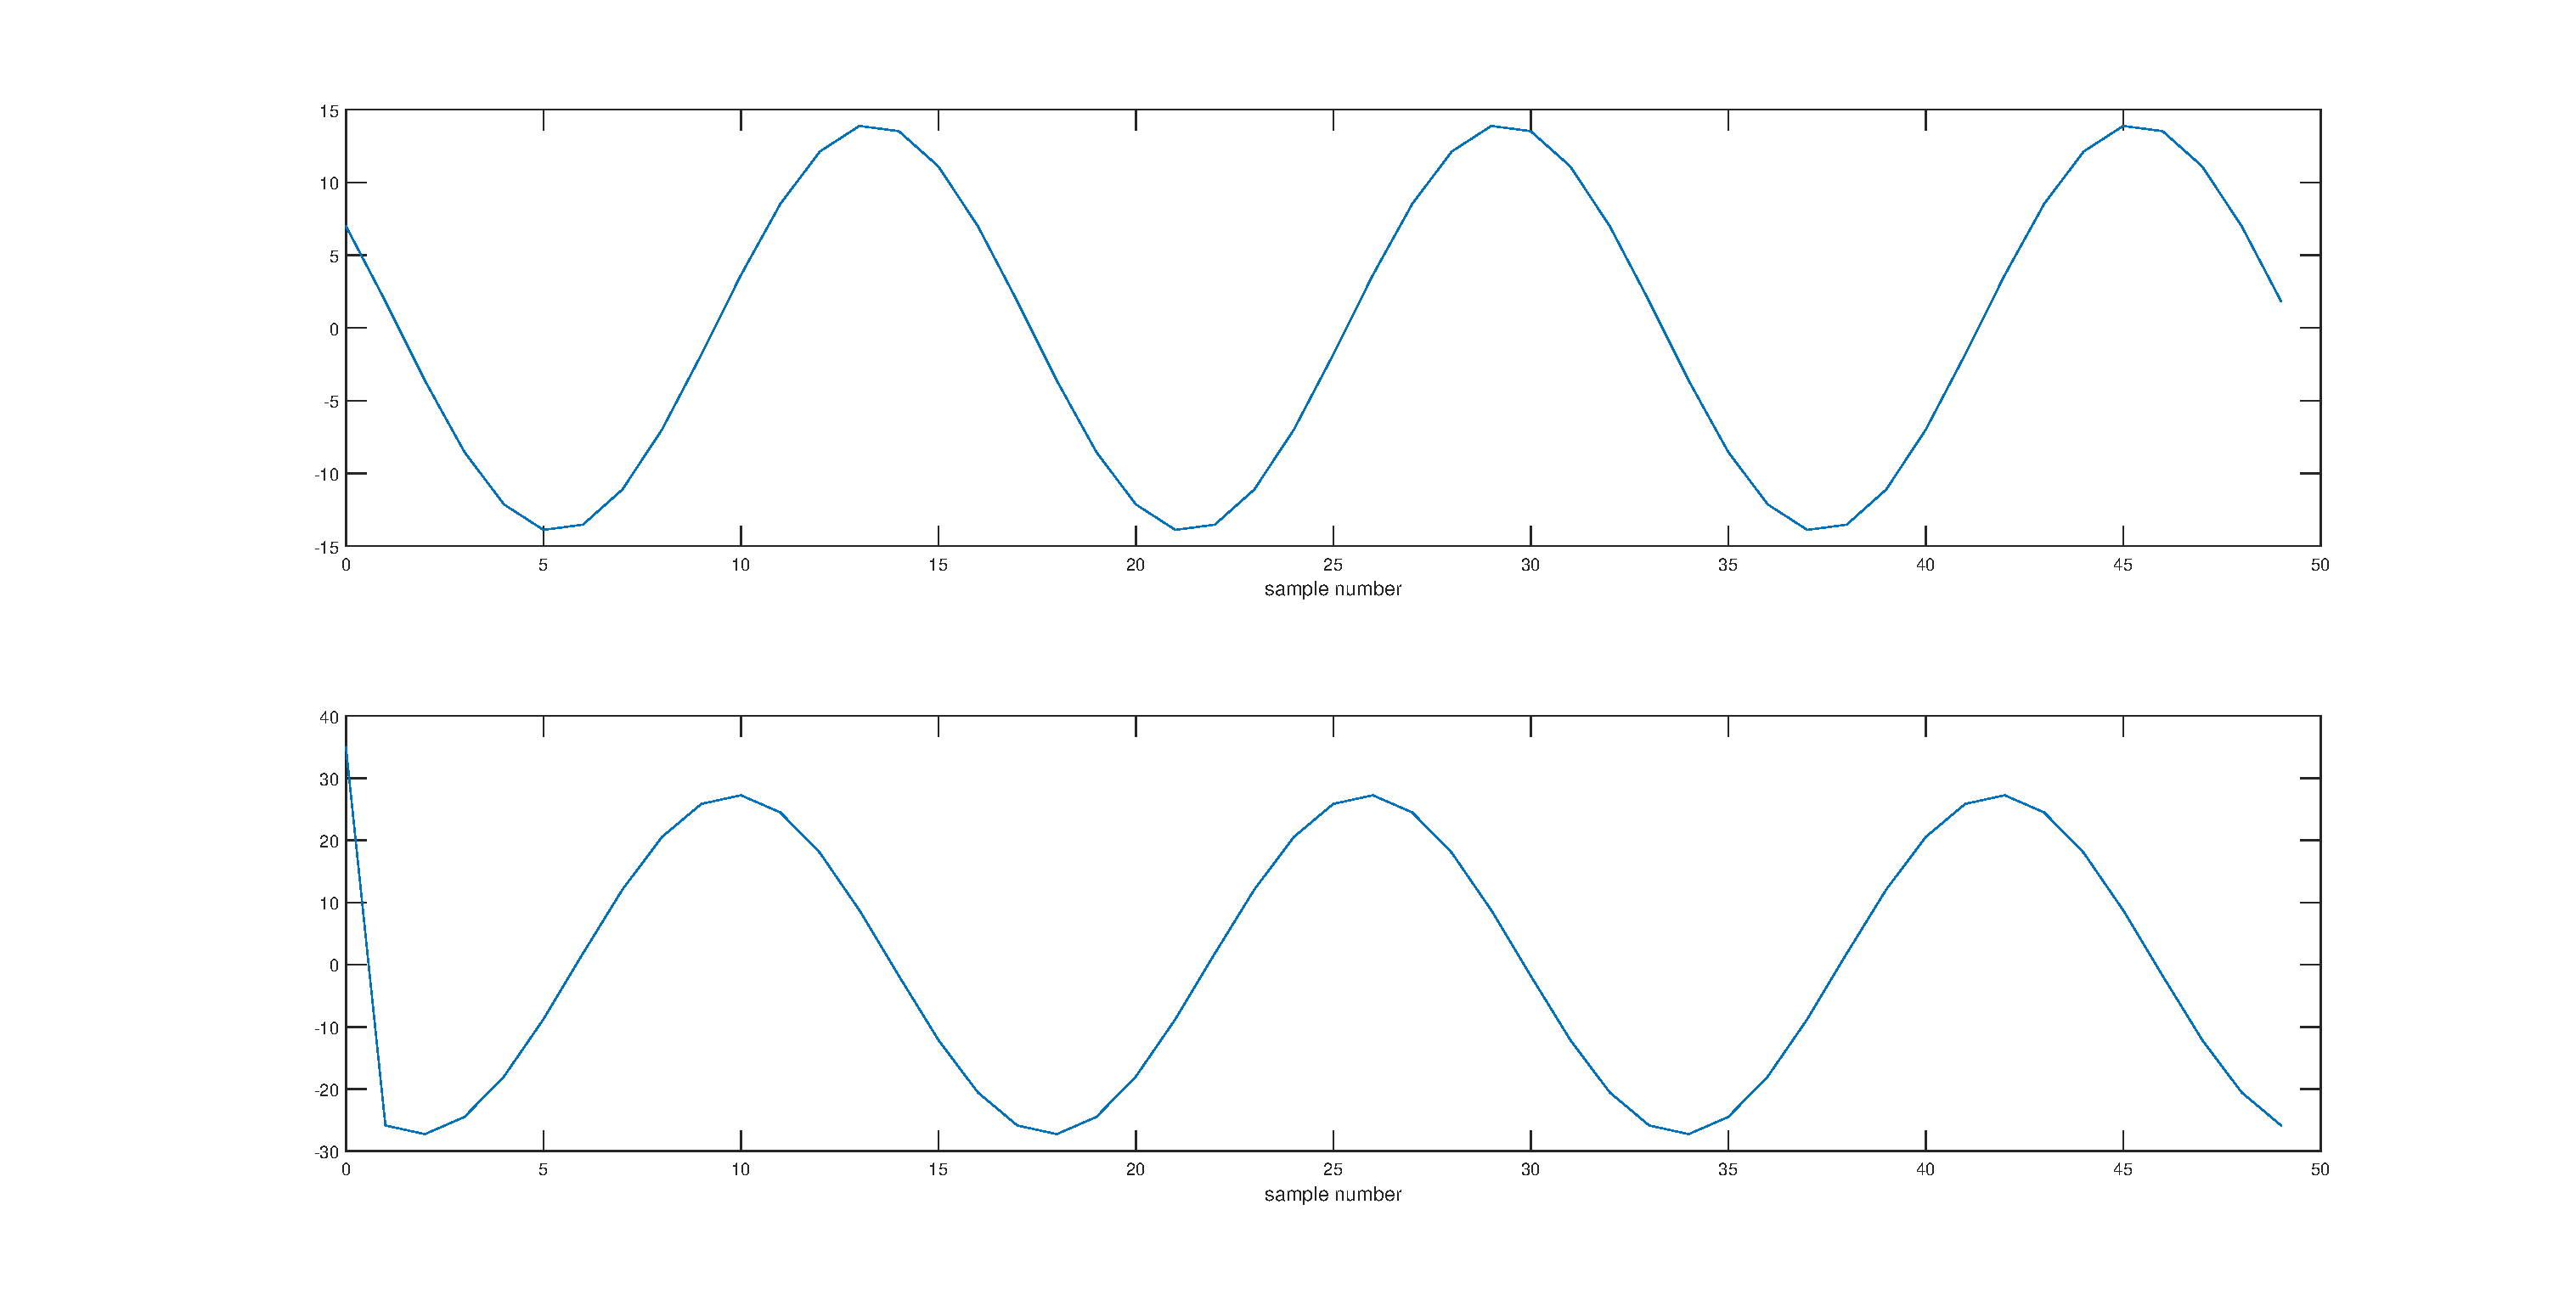
\includegraphics[scale=0.3]{fig4}
	\caption{Time series plot of input signal and filtered signal, using a first difference filter}
\end{figure}

\subsection{Part B}

If we instead input a signal $x[n] = 8 \cdot \cos(0.25 \pi)$, the implementation code would look like:
\begin{lstlisting}
	%%%%%%%%%%%%% 3.3 Linearity of the Filter %%%%%%%%%%%%%%%%%%
	
	% Clear the worksapce and any stored variables
	clear; clc;
	
	L = 50;
	
	% Create a vector which will be used to create samples
	nn = 0:(L-1);
	
	% Initialise the parameters used to define the input signal
	A = 8;
	ph = 0;
	ww = 0.25*pi;
	
	% Take discrete samples of the cosine
	xb = A*cos(ww*nn + ph);
	
	% Create the filter and the associated response to teh input signal
	bb = [5 -5];
	yb = firfilt(bb,xb);
	
	% Create plots to compare the inpust signal with the output signal
	subplot(2,1,1)
	plot(nn,xb)
	xlabel('sample number')
	
	subplot(2,1,2)
	plot(nn,yb(1:50))
	xlabel('sample number')
\end{lstlisting}

The time series plot of the input and output signals can be seen in Figure 5. We note that the amplitude of the input signal is 8, and the amplitude of the output signal is approximately 28. This gives the filter a gain of 3.5 at the discrete frequency of the input signal of $0.25 \pi$. The phase shift for the input signal is zero, and the phase shift for the output signal is 2 sample points, which equates to a phase shift of $\frac{\pi}{2}$. Hence the phase shift of the frequency response function is $\frac{\pi}{2}$.

\begin{figure}[H]
	\centering
	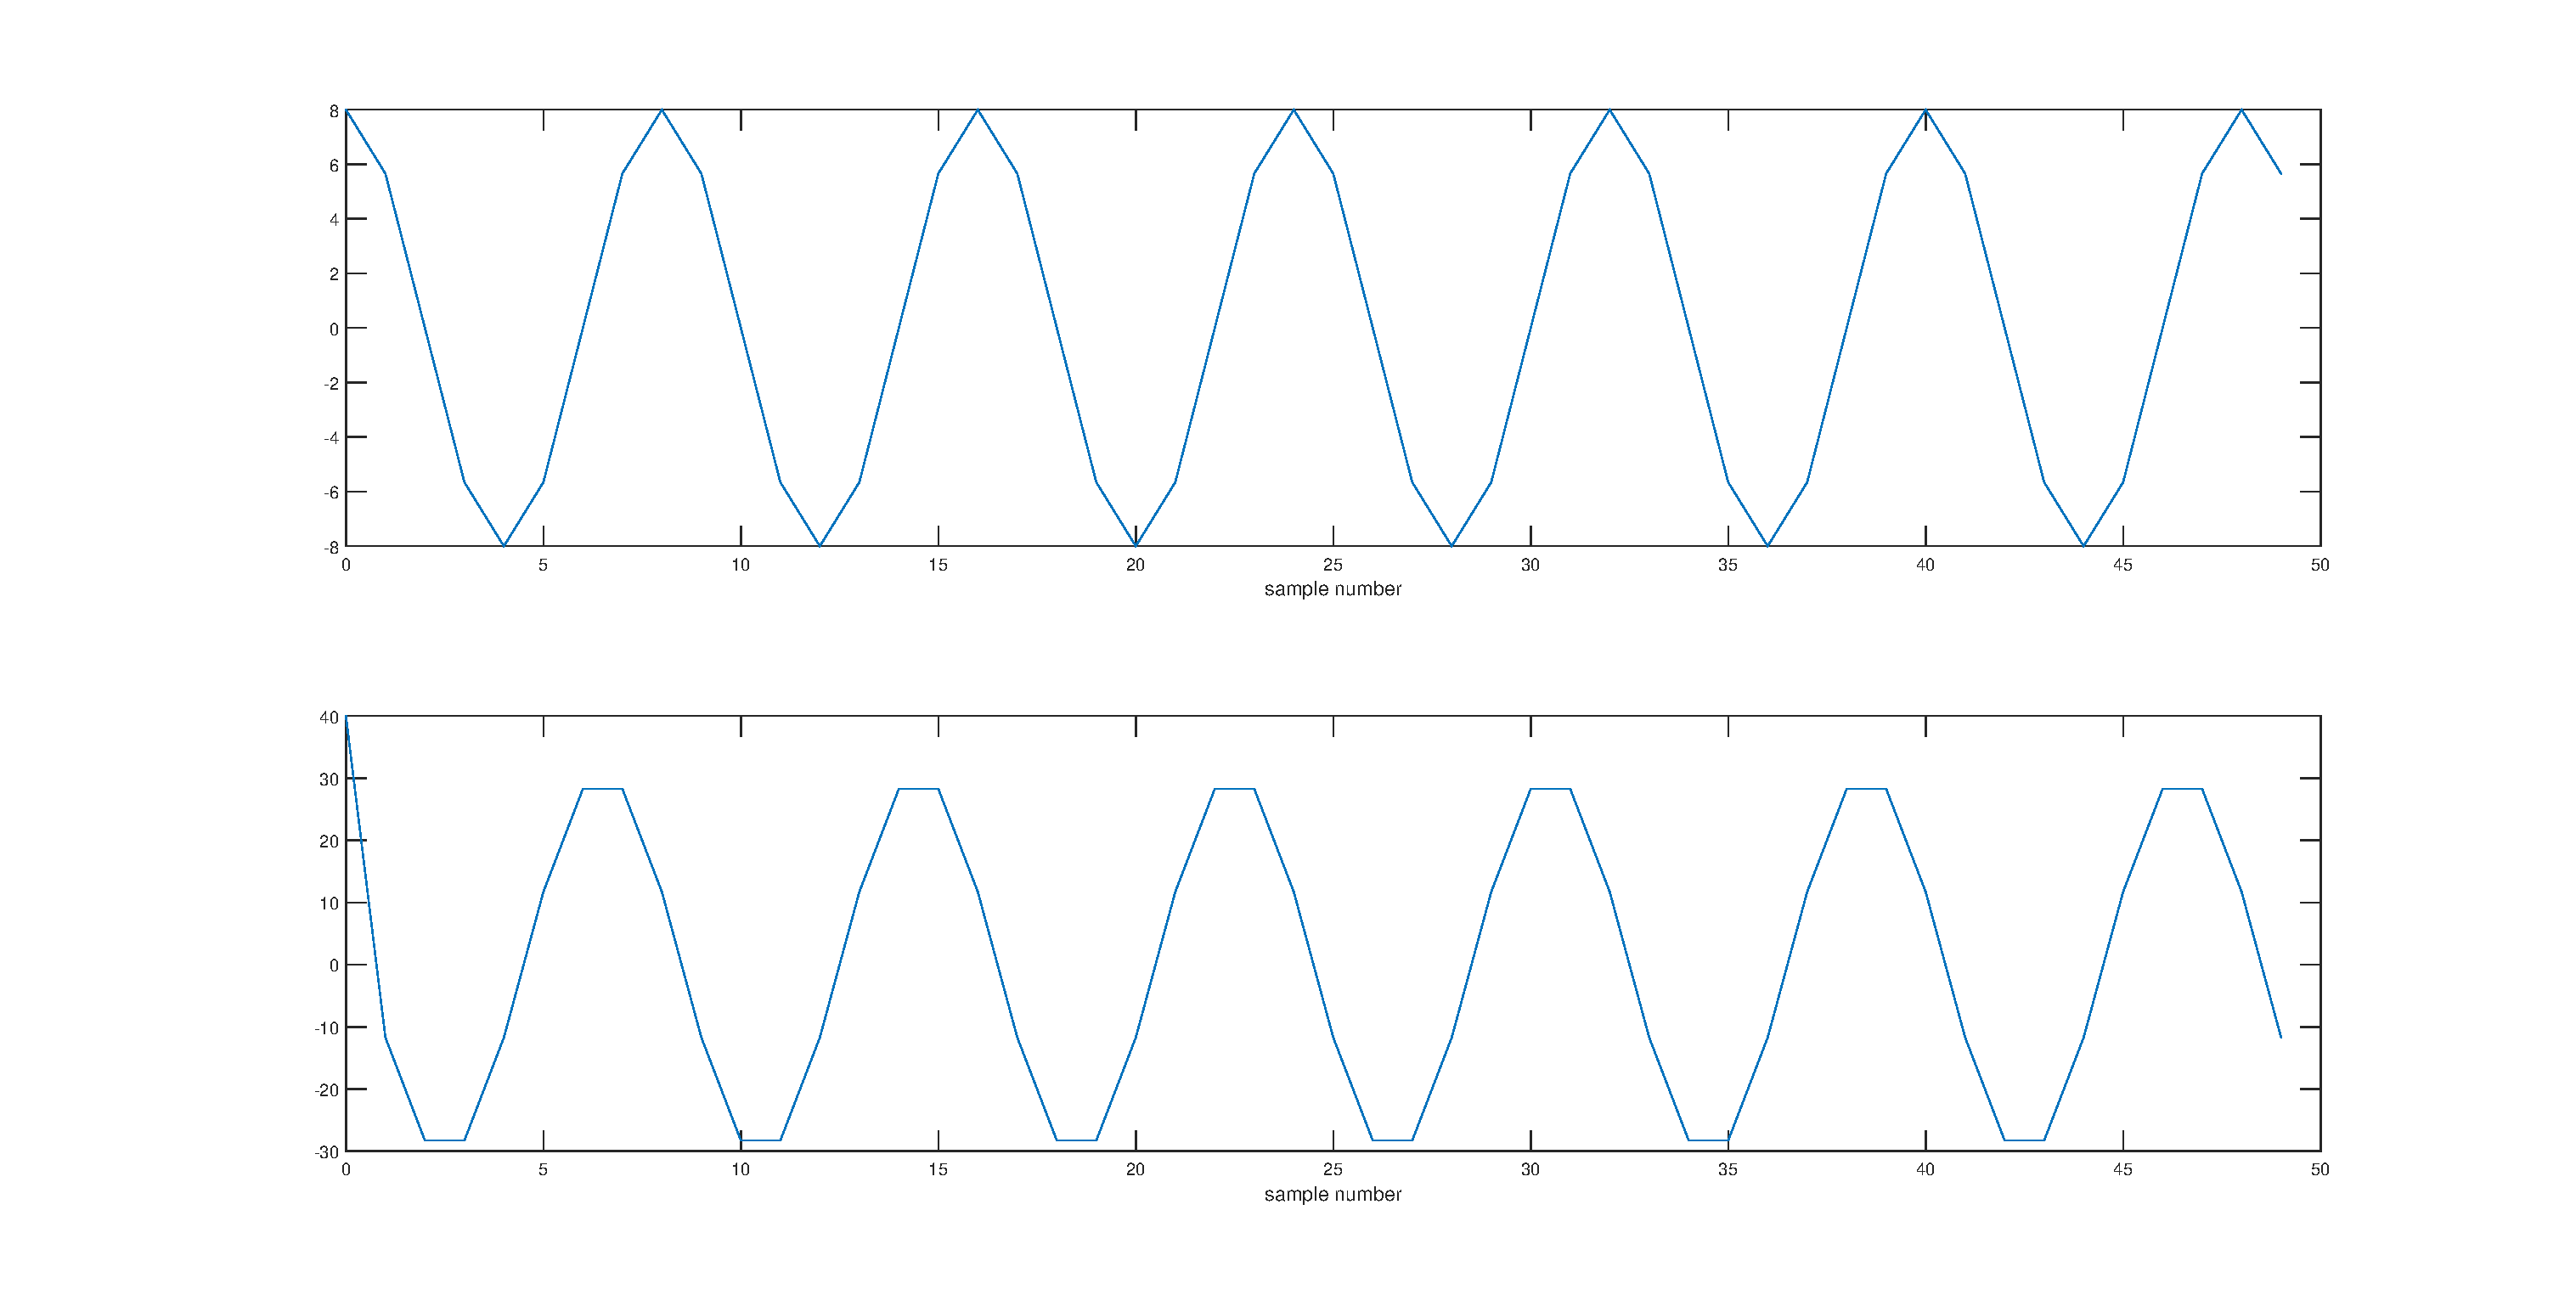
\includegraphics[scale=0.3]{fig5}
	\caption{Time series plot of input signal and filtered signal, using a first difference filter}
\end{figure}

\subsection{Part C}
Finally, another input signal was formed by linearly adding the previous two input signals:
\begin{align*}
	x[n] = 7 \cdot \cos(0.125 \pi n + \sfrac{\pi}{3}) + 8 \cdot \cos(0.25 \pi n)
\end{align*}

The new signal was input to the first difference filter. This was implemented using MATLAB:
\begin{lstlisting}
	%%%%%%%%%%%%%% 3.3 Linearity of the Filter %%%%%%%%%%%%%%%%%
	
	% Clear the worksapce and any stored variables
	clear; clc;
	
	L = 50;
	
	% Create a vector which will be used to create samples
	nn = 0:(L-1);
	
	% Initialise the parameters used to define the input signal xa
	A_a = 7;
	ph_a = pi/3;
	ww_a = 0.125*pi;
	
	% Take discrete samples of the cosine
	xx = A_a*cos(ww_a*nn + ph_a);
	
	% Create a linearly scaled version of xx
	xa = 2*xx;
	
	% Initialise the parameters used to define the input signal xb
	A_b = 8;
	ph_b = 0;
	ww_b = 0.25*pi;
	
	% Take discrete samples of the cosine
	xb = A_b*cos(ww_b*nn + ph_b);
	
	% Create an additive signal
	xc = xa + xb;
	
	% Create the filter and the associated response to teh input signal
	bb = [5 -5];
	yc = firfilt(bb,xc);
	
	% Create plots to compare the inpust signal with the output signal
	subplot(2,1,1)
	plot(nn,xc)
	
	subplot(2,1,2)
	plot(nn,yc(1:50))
\end{lstlisting}

The output time series plots can be seen in Figure 6. More importantly, we can see an output graph in Figure 7 which shows the output signal from this additive input on the bottom plot, and the output signal after passing the two input signals through the filter independently and adding the two results afterwards. These two plots look identical. This is an important result, it shows us that this is a linear filter.

\begin{figure}[H]
	\centering
	\begin{minipage}[t]{0.4\linewidth}
		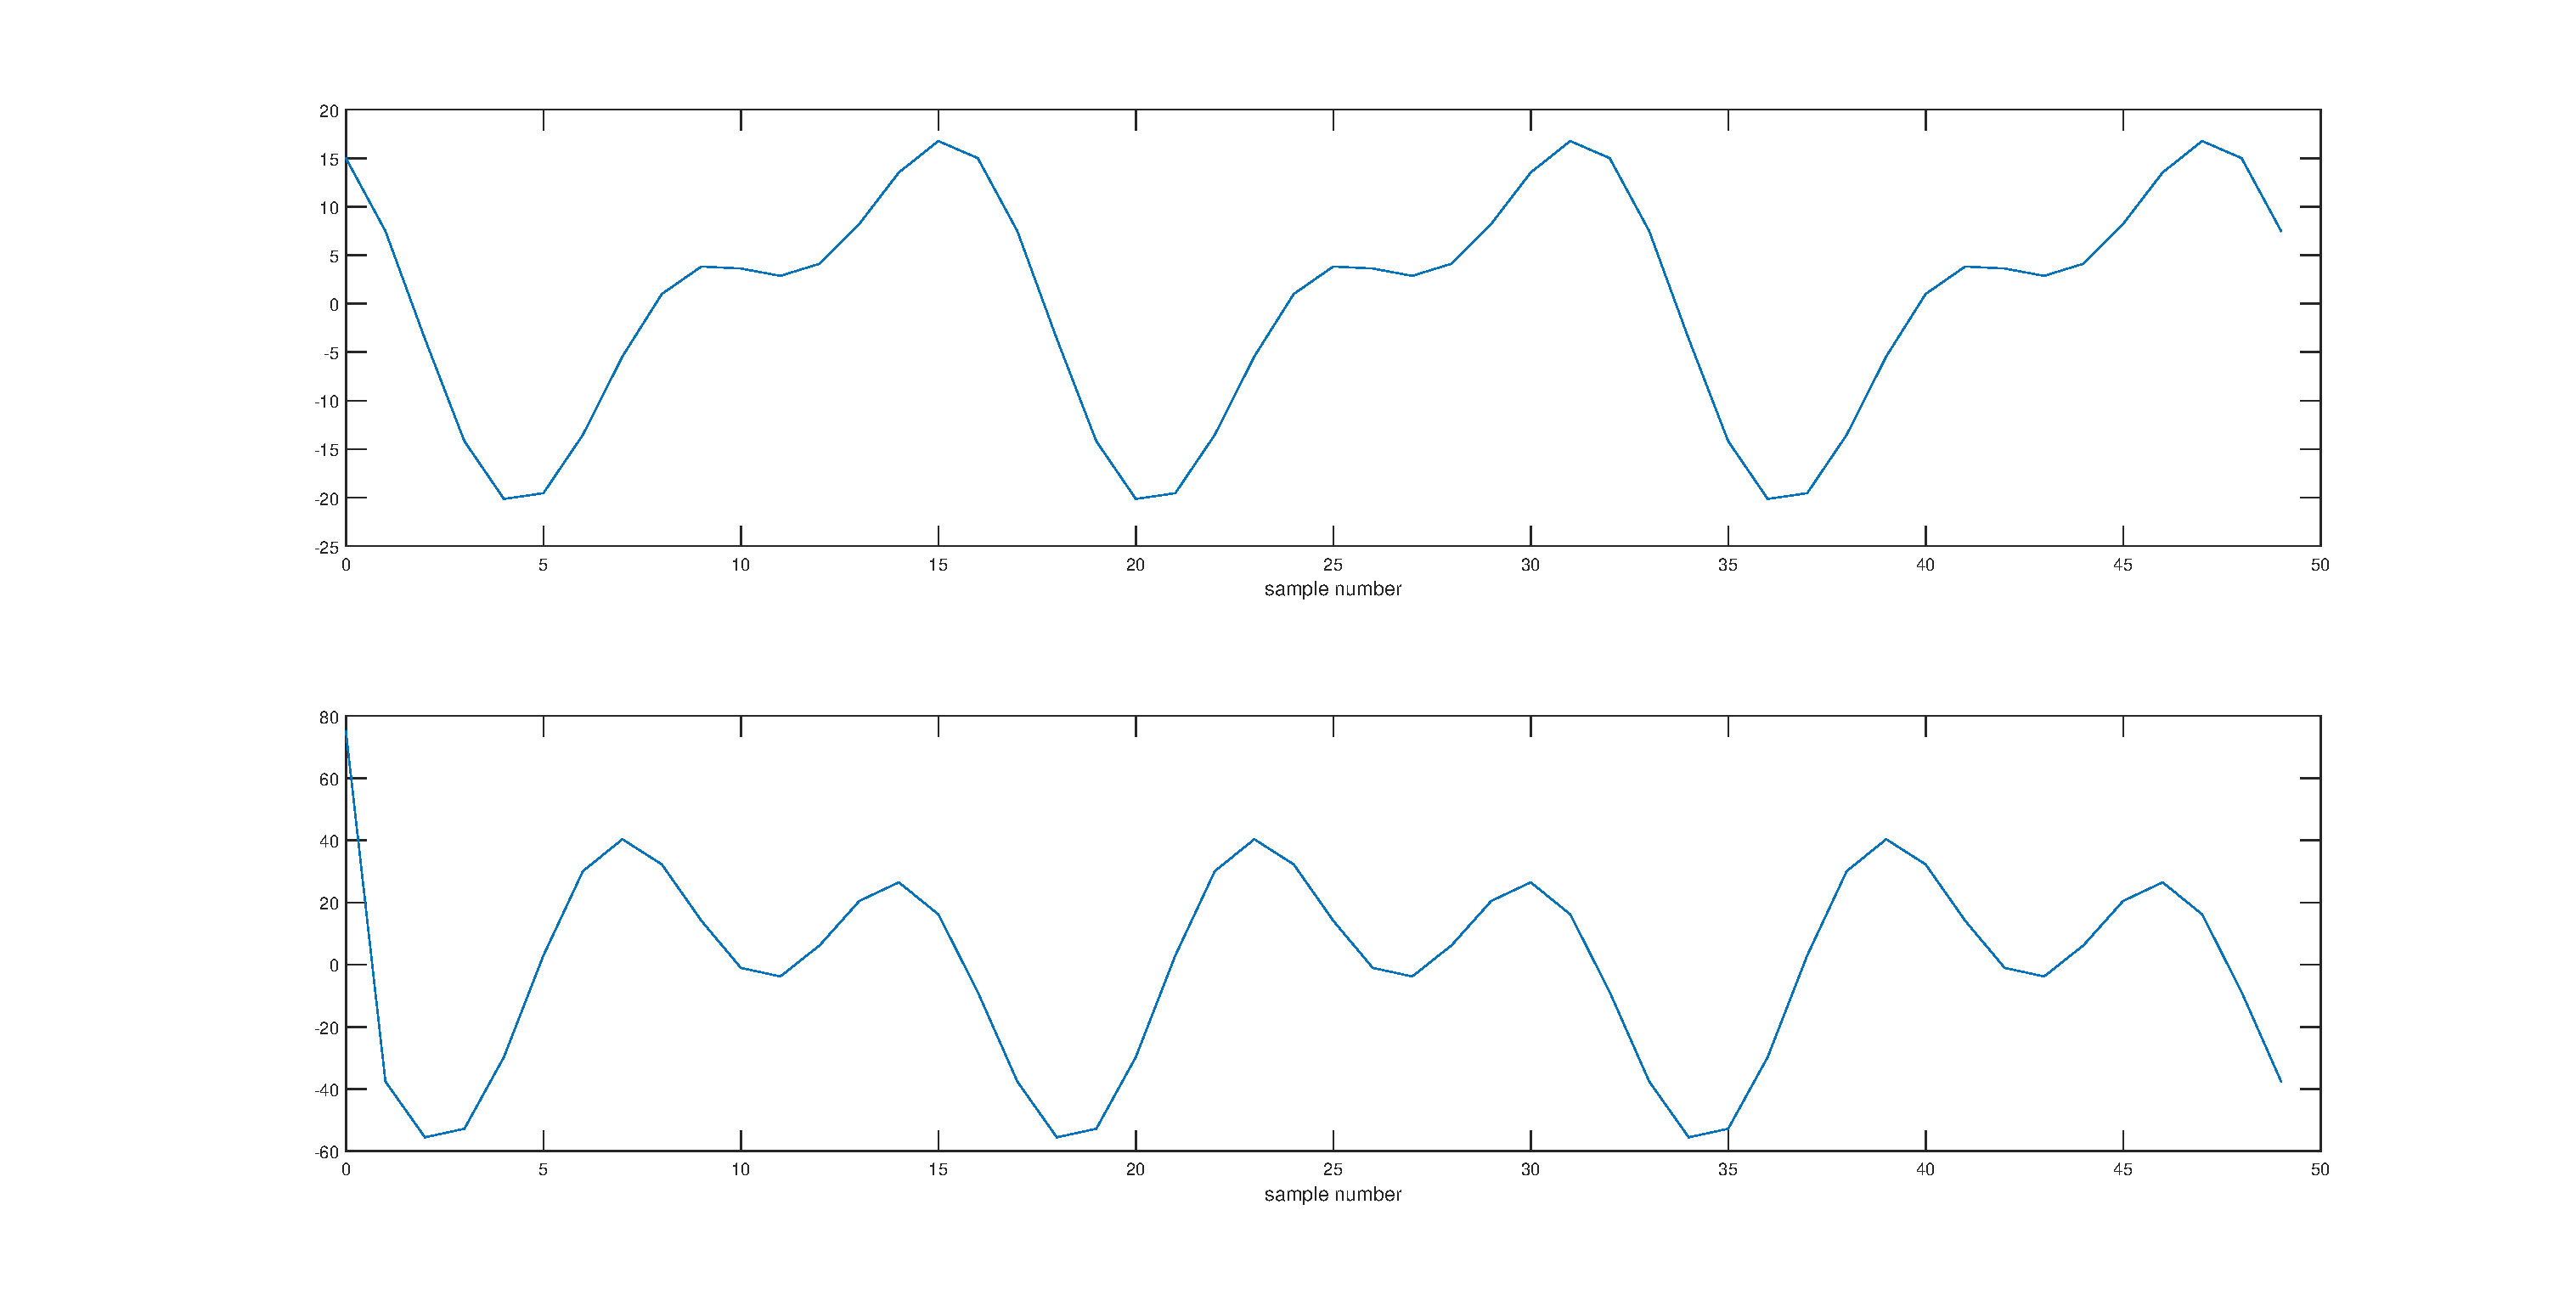
\includegraphics[scale=0.15]{fig6}
		\caption{A time series plot of the additive input signal shown on the top and the filtered output signal shown on the bottom}
	\end{minipage}
	\hspace{2cm}
	\begin{minipage}[t]{0.4\linewidth}
		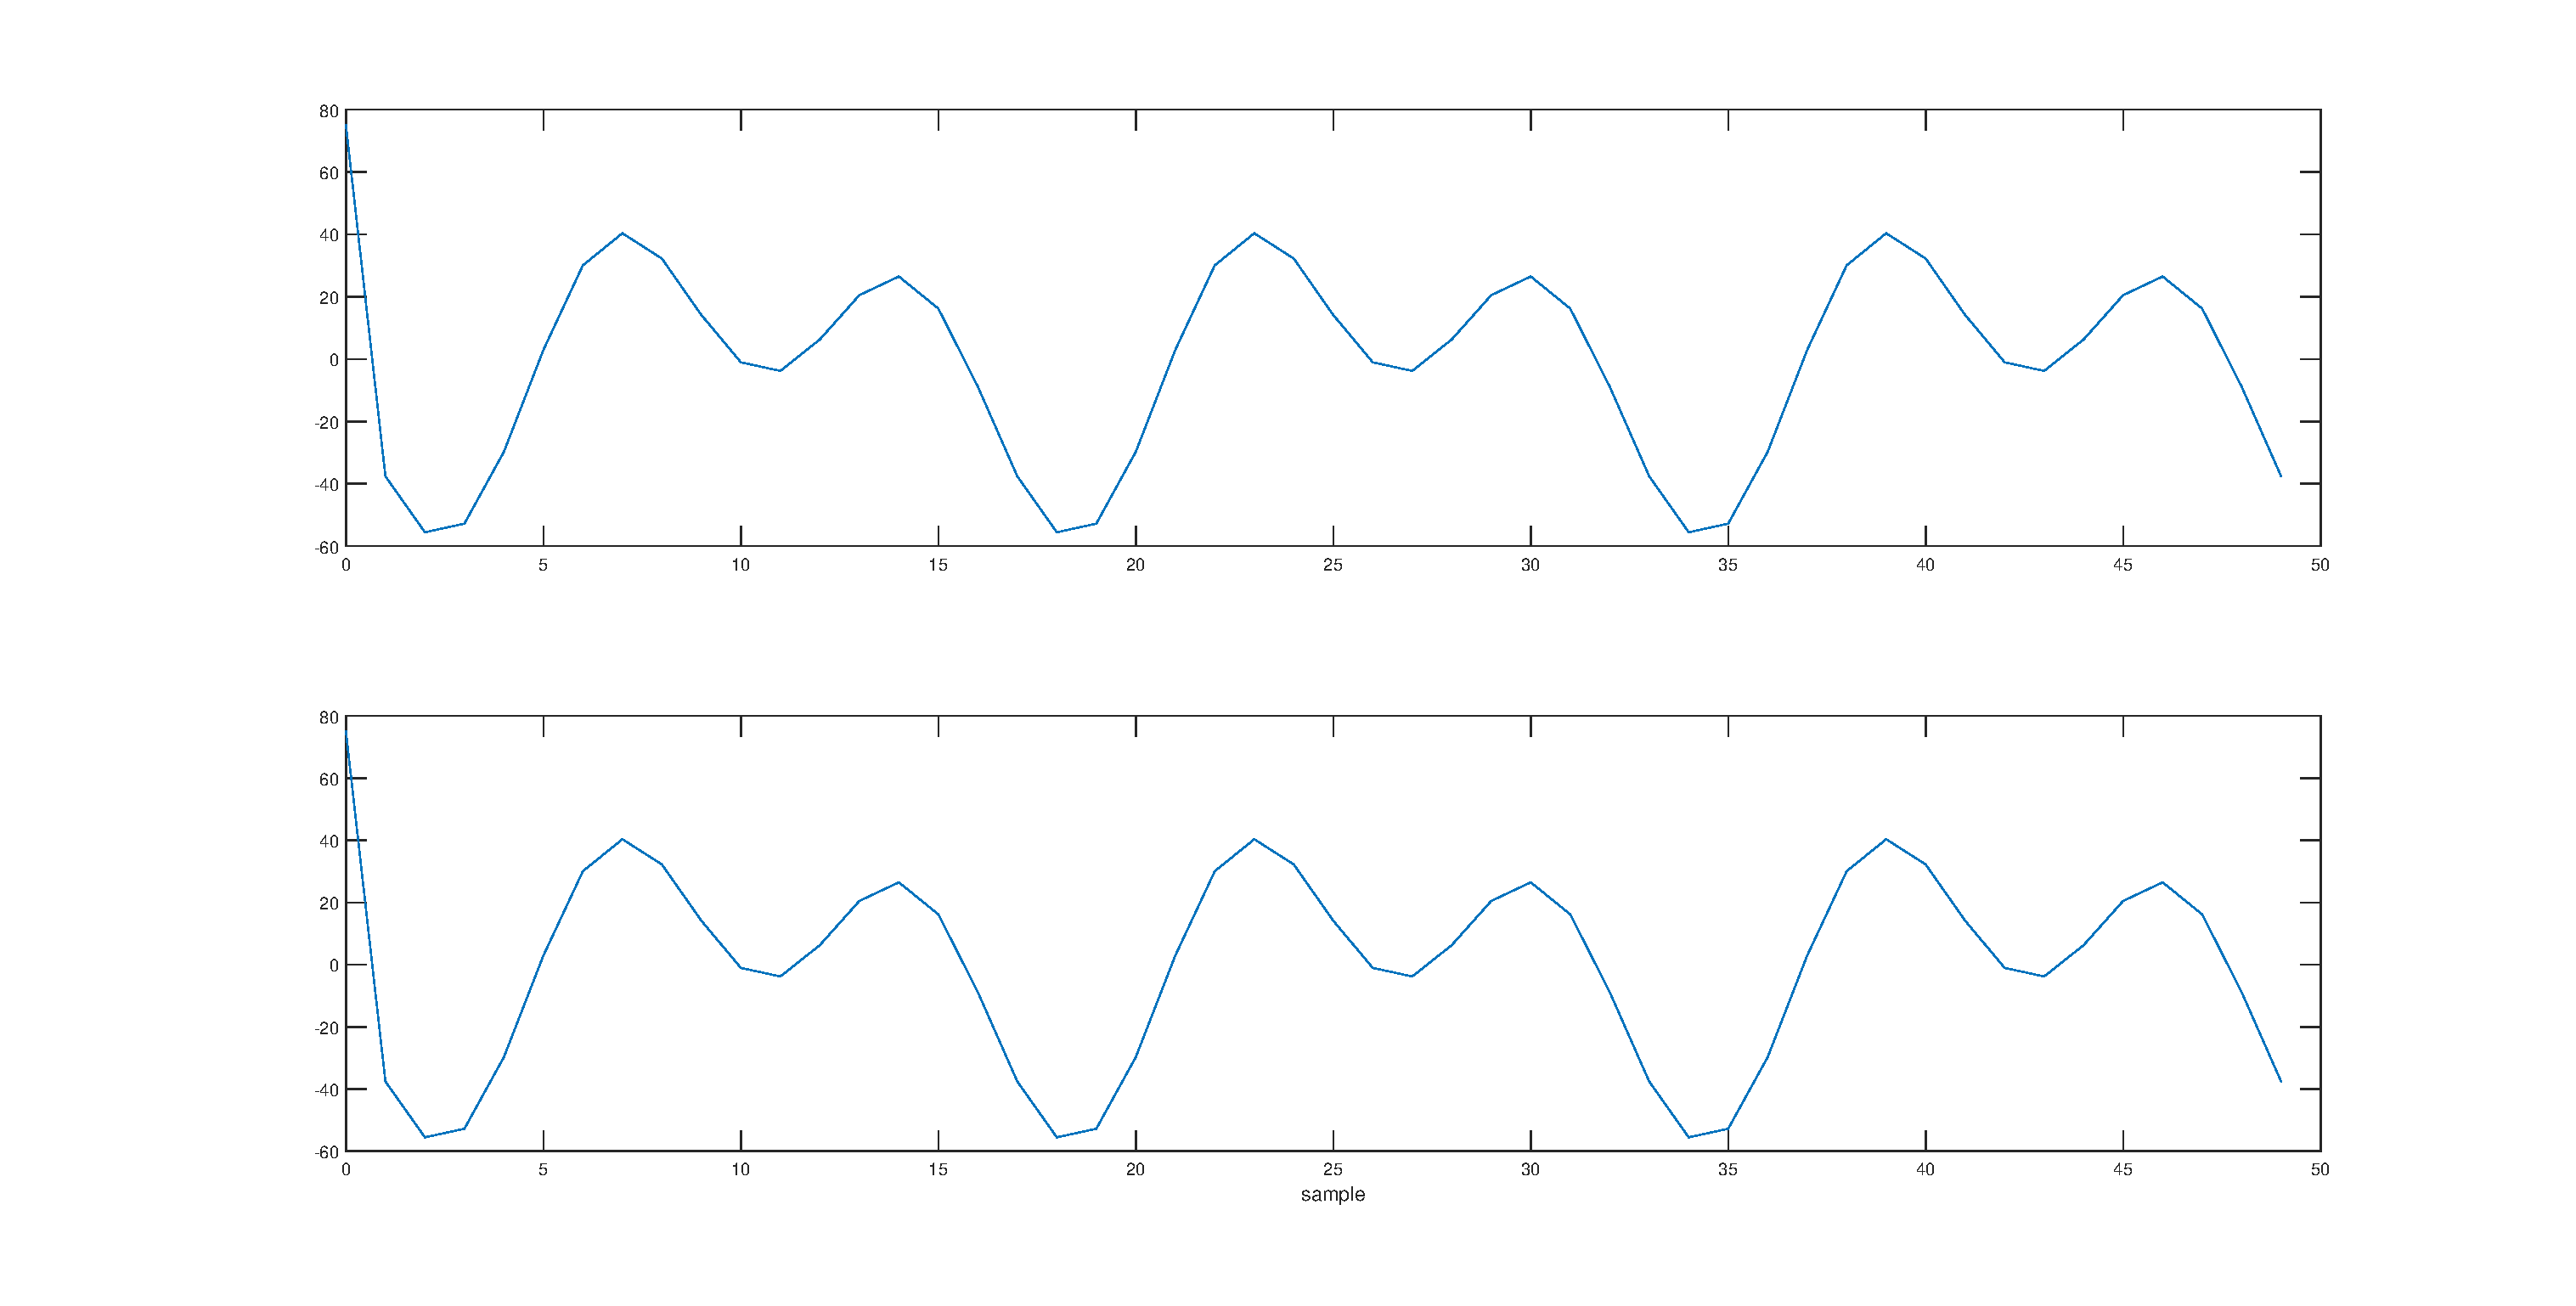
\includegraphics[scale=0.15]{fig7}
		\caption{A time series plot of the output signal from the additive input is shown above, and the separate outputs from the previous two experiments summed together shown on the bottom plot}
	\end{minipage}
\end{figure}

\section{3.4 Time-Invariance of the Filter}

Consider the following signal:
\begin{align*}
	x[n] = 7 \cdot \cos(0.125 \pi \cdot (n - 3) + \sfrac{\pi}{3})
\end{align*}

The signal shown above was implemented in MATLAB and passed through a first difference filter, as shown:
\begin{lstlisting}
	%%%%%%%%%%%%%%% 3.4 Time-Invariance of the Filter %%%%%%%%%%%%%%%%%%%
	
	% Clear the workspace and clear any stored variables
	clear; clc;
	
	L = 50;
	
	% Create a vector which will be used to create samples
	nn = 0:(L-1);
	
	% Initialise the parameters used to define the input signal xa
	A_a = 7;
	ph_a = pi/3;
	ww_a = 0.125*pi;
	
	% Take discrete samples of the cosine
	xs = A_a*cos(ww_a*(nn-3) + ph_a);
	
	% Create the filter and the associated response to teh input signal
	bb = [5 -5];
	ys = firfilt(bb,xs);
	
	% Create plots to compare the inpust signal with the output signal
	subplot(2,1,1)
	plot(nn,xs)
	xlabel('sample')
	
	subplot(2,1,2)
	plot(nn,ys(1:50))
	xlabel('sample')
\end{lstlisting}

The plot can be seen in Figure 8 below. From the graph it can be seen that the shift in the number of samples is 3.

\begin{figure}[H]
	\centering
	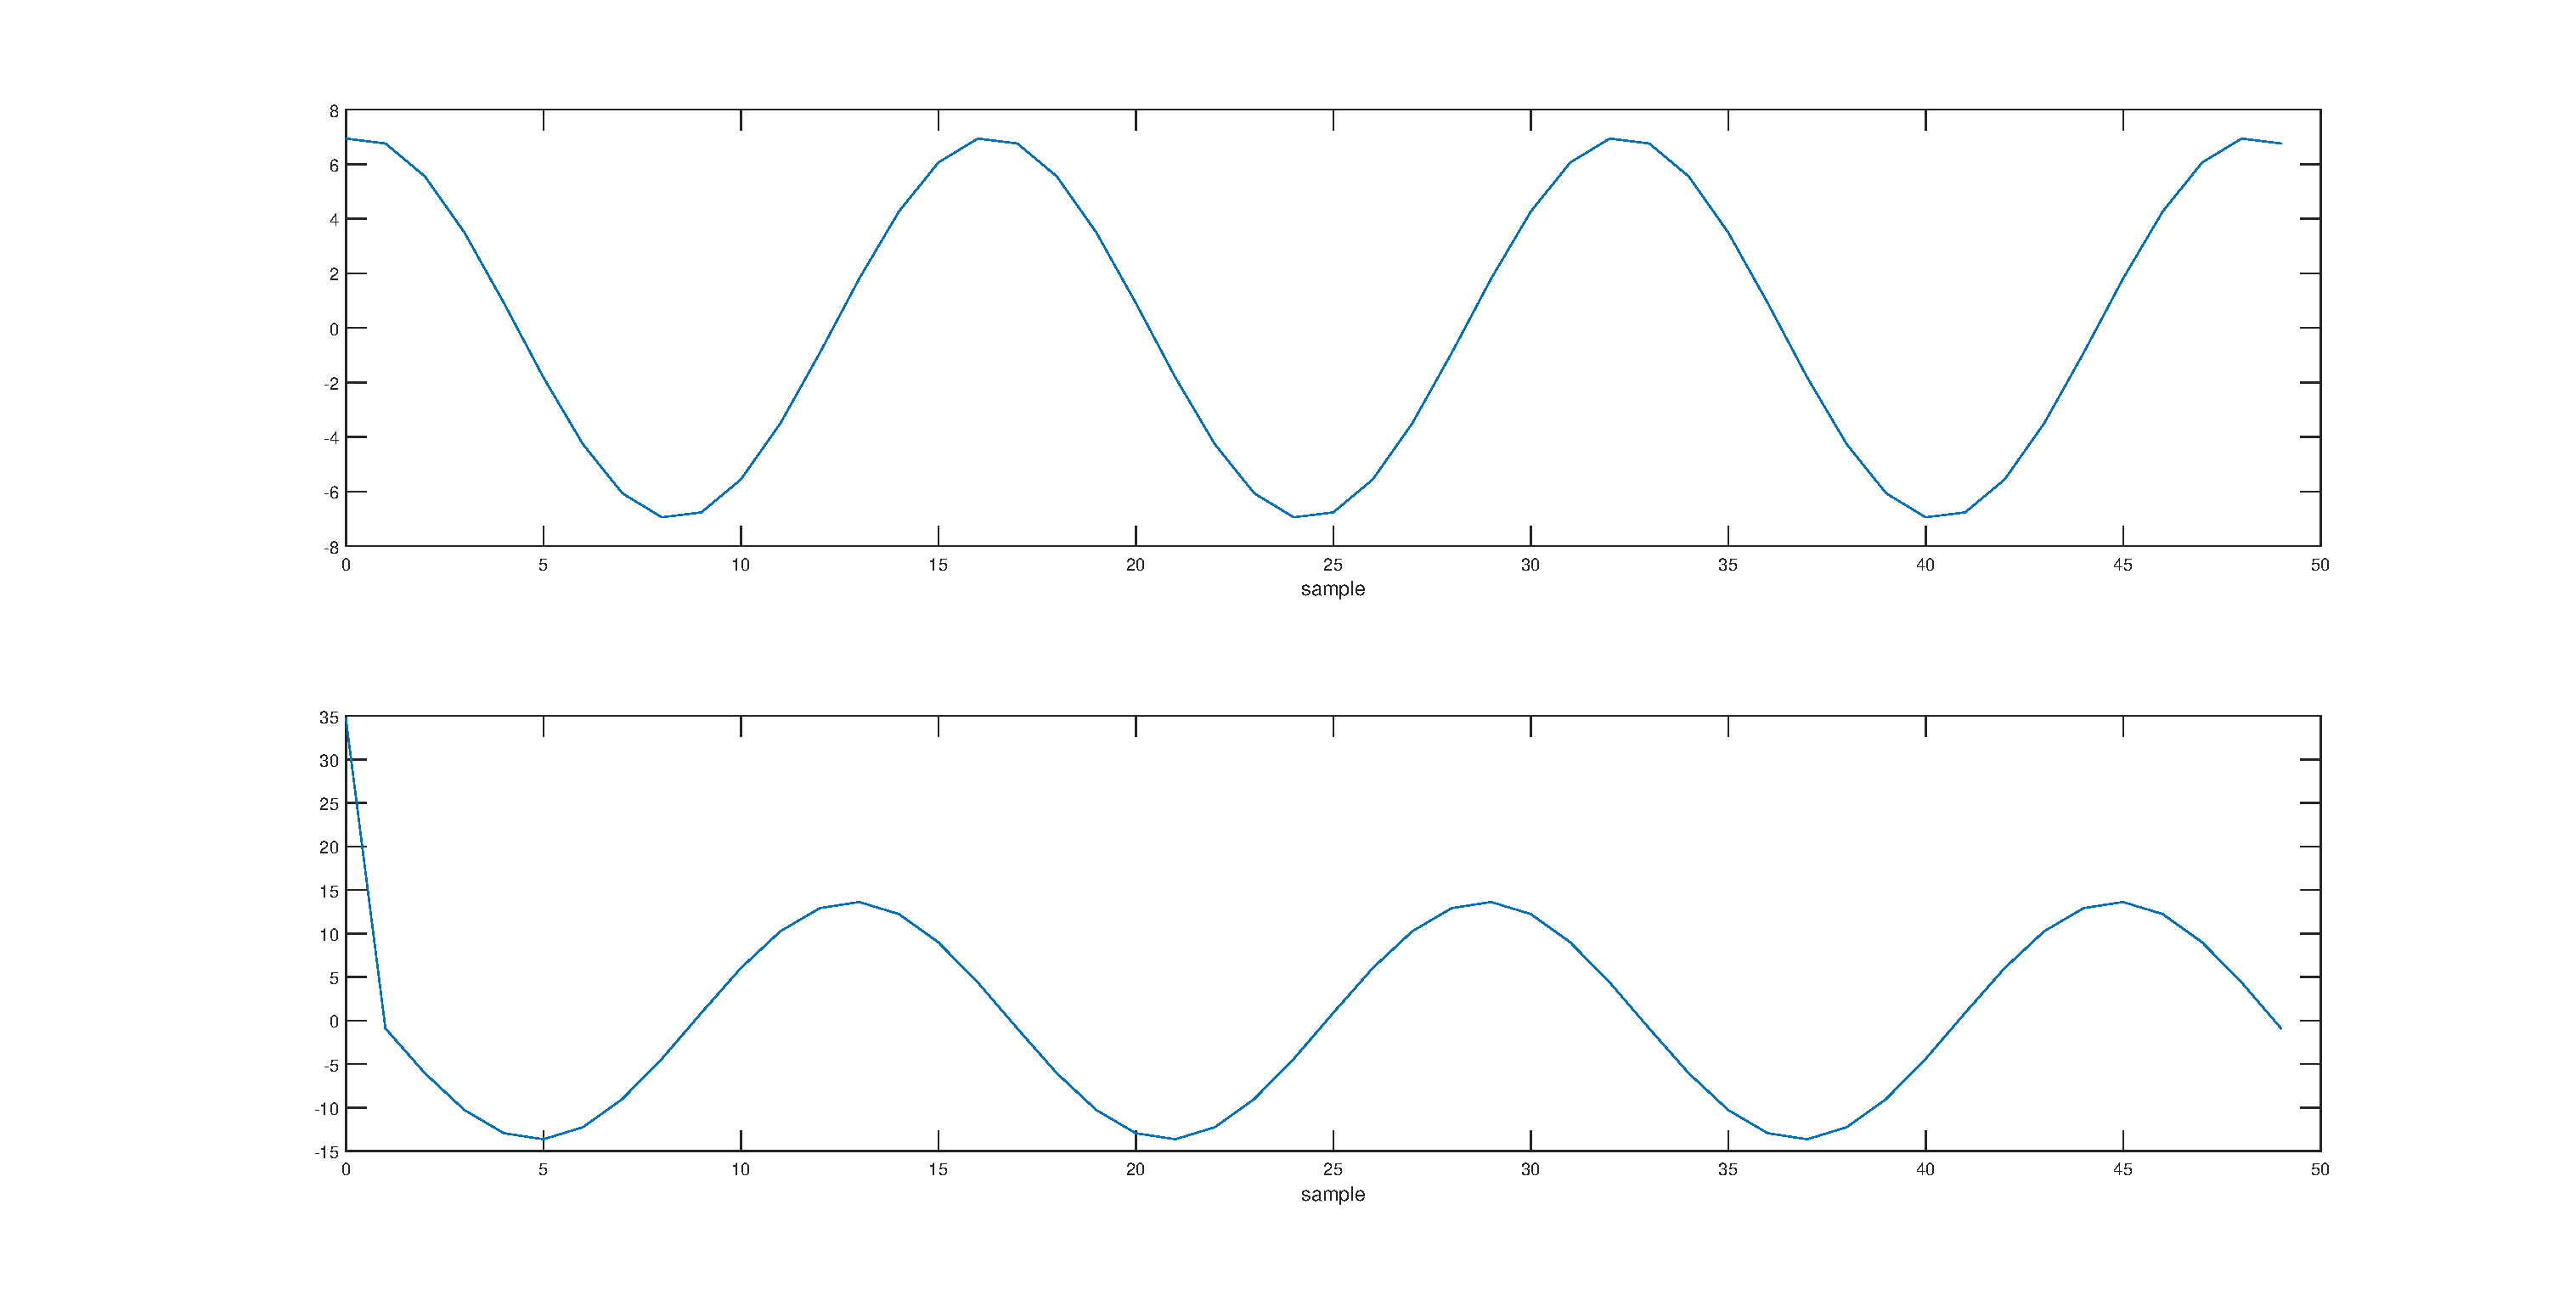
\includegraphics[scale=0.3]{fig8}
	\caption{Time shifted response (below) to the input signal (above).}
\end{figure}

\section{3.5 Cascading Two Systems}

A MATLAB implementation of the code can be found below:
\begin{lstlisting}
	%%%%%%%%%%%%%%%%% 3.5 Cascading Two Systems Part 2 %%%%%%%%%%%%%%%%%%%
	
	% Clear the workspace and any stored variables
	clear; clc;
	
	L = 50;
	
	% Create a vector which will be used to create samples
	nn = 0:(L-1);
	
	% Initialise the parameters used to define the input signal
	A = 7;
	ph = pi/3;
	ww = 0.125*pi;
	
	% Take discrete samples of the cosine
	xx = A*cos(ww*nn + ph);
	
	% Passing the signal through the squaring filter
	ww = xx.^2;
	
	% Create pass the squared signal through a differencing filter
	bb = [1,-2*cos(0.25*pi),1];
	yy = firfilt(bb,ww);
	
	% Create plots to compare the inpust signal with the output signal
	figure(1)
	subplot(3,1,1)
	plot(nn,xx)
	
	subplot(3,1,2)
	plot(nn,ww)
	
	subplot(3,1,3)
	plot(nn,yy(1:50))
	
	figure(2)
	subplot(3,1,1)
	specgram(xx)
	subplot(3,1,2)
	specgram(ww)
	subplot(3,1,3)
	specgram(yy)
\end{lstlisting}

A plot of the original input signal, the squared signal and the final output signal from the cascaded system can be seen in Figure 9. Further Figure 10 shows the spectrograms of each of the signals.

\begin{figure}[H]
	\centering
	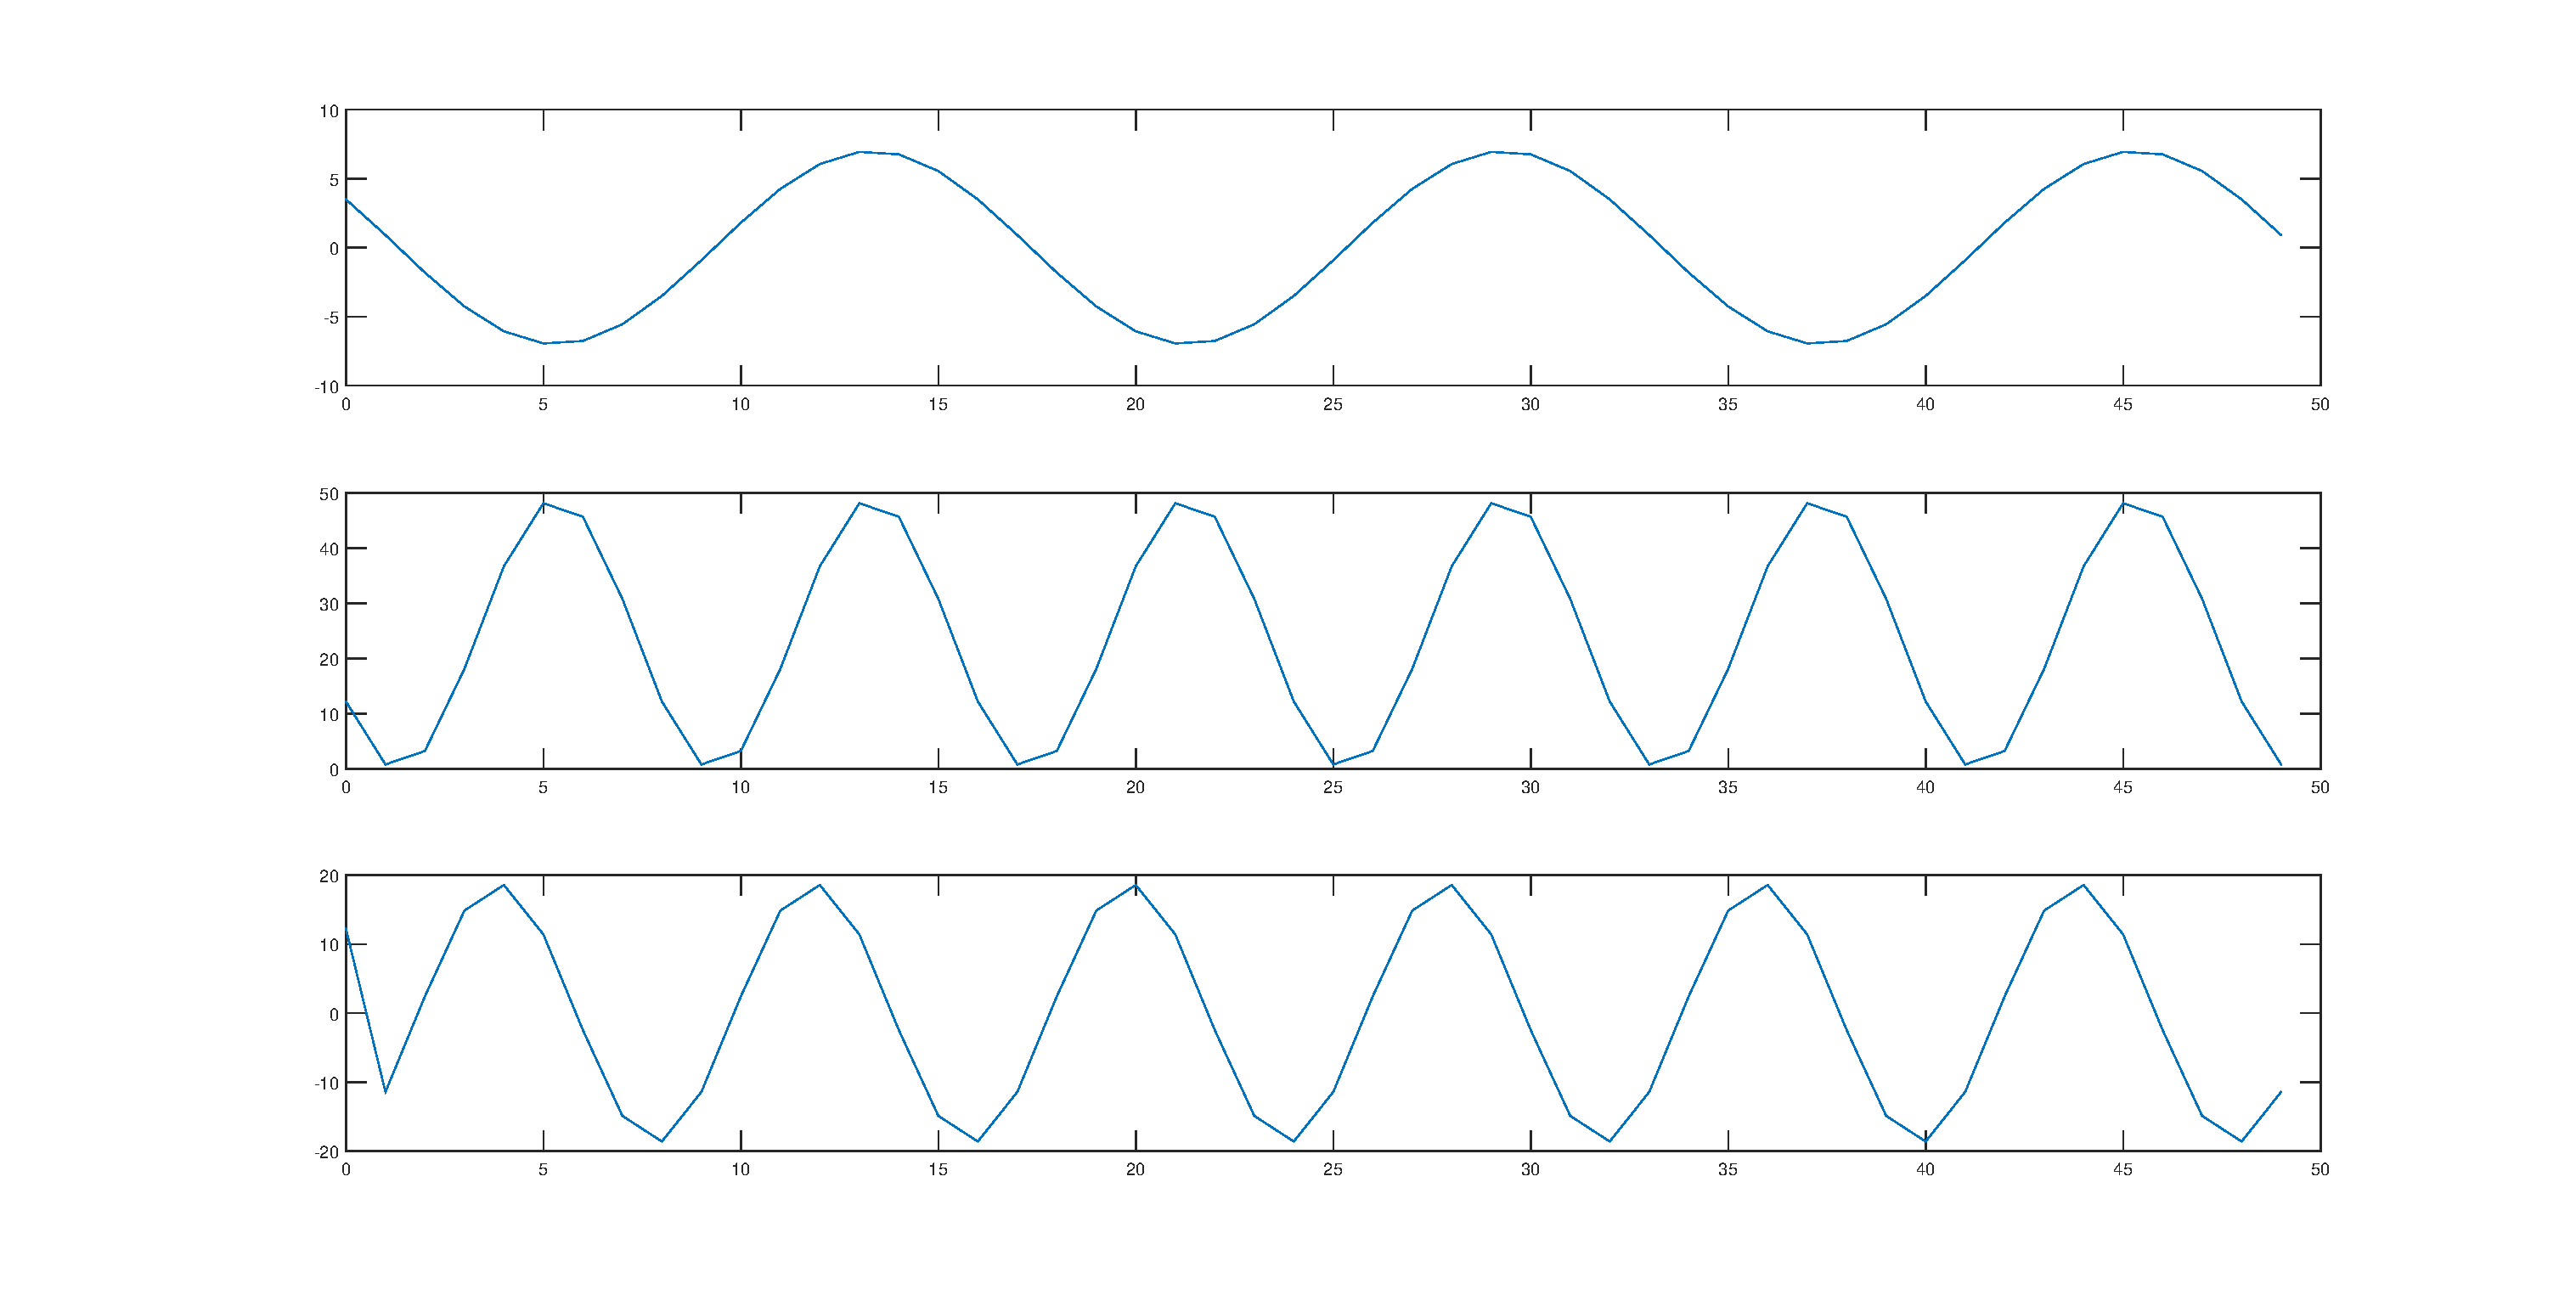
\includegraphics[scale=0.25]{fig9}
	\caption{Time series plot of the input signal, the squared signal and the final signal after the squared signal is passed through the first difference filter}
\end{figure}

\begin{figure}[H]
	\centering
	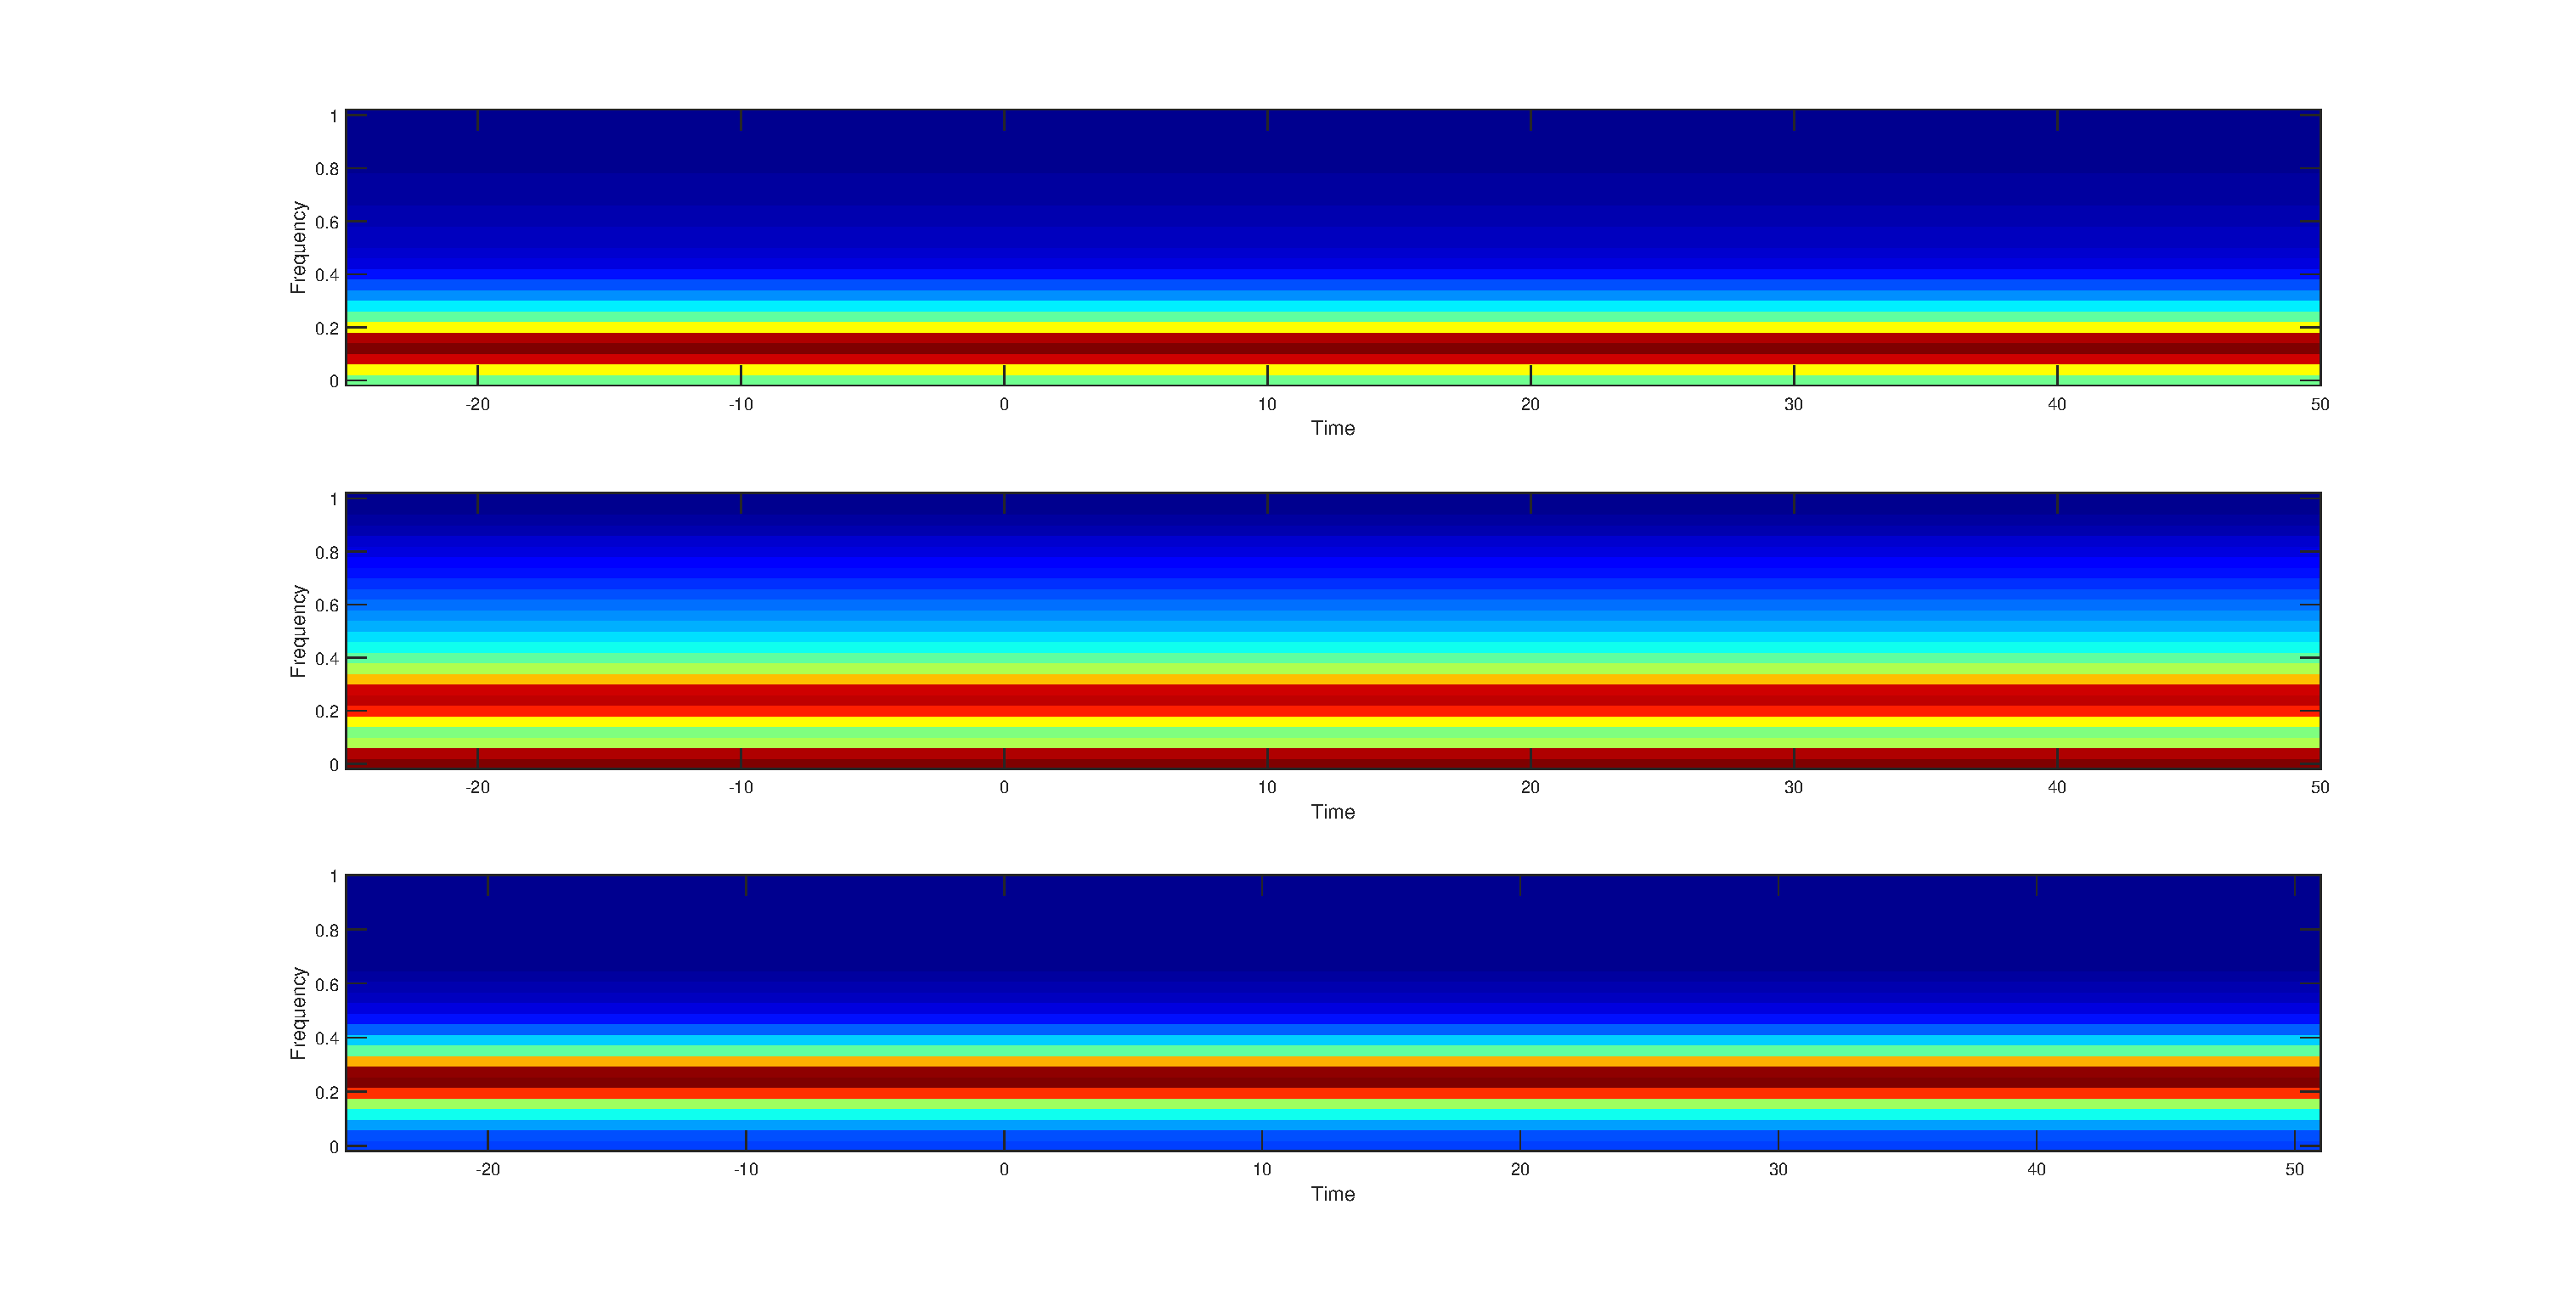
\includegraphics[scale=0.25]{fig10}
	\caption{A spectrogram of all three stages of signal}
\end{figure}

Finally, a second order filter was implemented. The following MATLAB code was used to implement the filter:
\begin{lstlisting}
	%%%%%%%%%%%%%%%%% 3.5 Cascading Two Systems Part 2 %%%%%%%%%%%%%%%%%%%
	
	% Clear the workspace and any stored variables
	clear; clc;
	
	L = 50;
	
	% Create a vector which will be used to create samples
	nn = 0:(L-1);
	
	% Initialise the parameters used to define the input signal
	A = 7;
	ph = pi/3;
	ww = 0.125*pi;
	
	% Take discrete samples of the cosine
	xx = A*cos(ww*nn + ph);
	
	% Passing the signal through the squaring filter
	ww = xx.^2;
	
	% Create pass the squared signal through a differencing filter
	bb = [1,-2*cos(0.25*pi),1];
	yy = firfilt(bb,ww);
	
	% Create plots to compare the inpust signal with the output signal
	figure(1)
	subplot(3,1,1)
	plot(nn,xx)
	
	subplot(3,1,2)
	plot(nn,ww)
	
	subplot(3,1,3)
	plot(nn,yy(1:50))
	
	figure(2)
	subplot(3,1,1)
	specgram(xx)
	subplot(3,1,2)
	specgram(ww)
	subplot(3,1,3)
	specgram(yy)
\end{lstlisting}

Figures 11 and 12 show the time series plot and the spectrogram, respectively.

\begin{figure}[H]
	\centering
	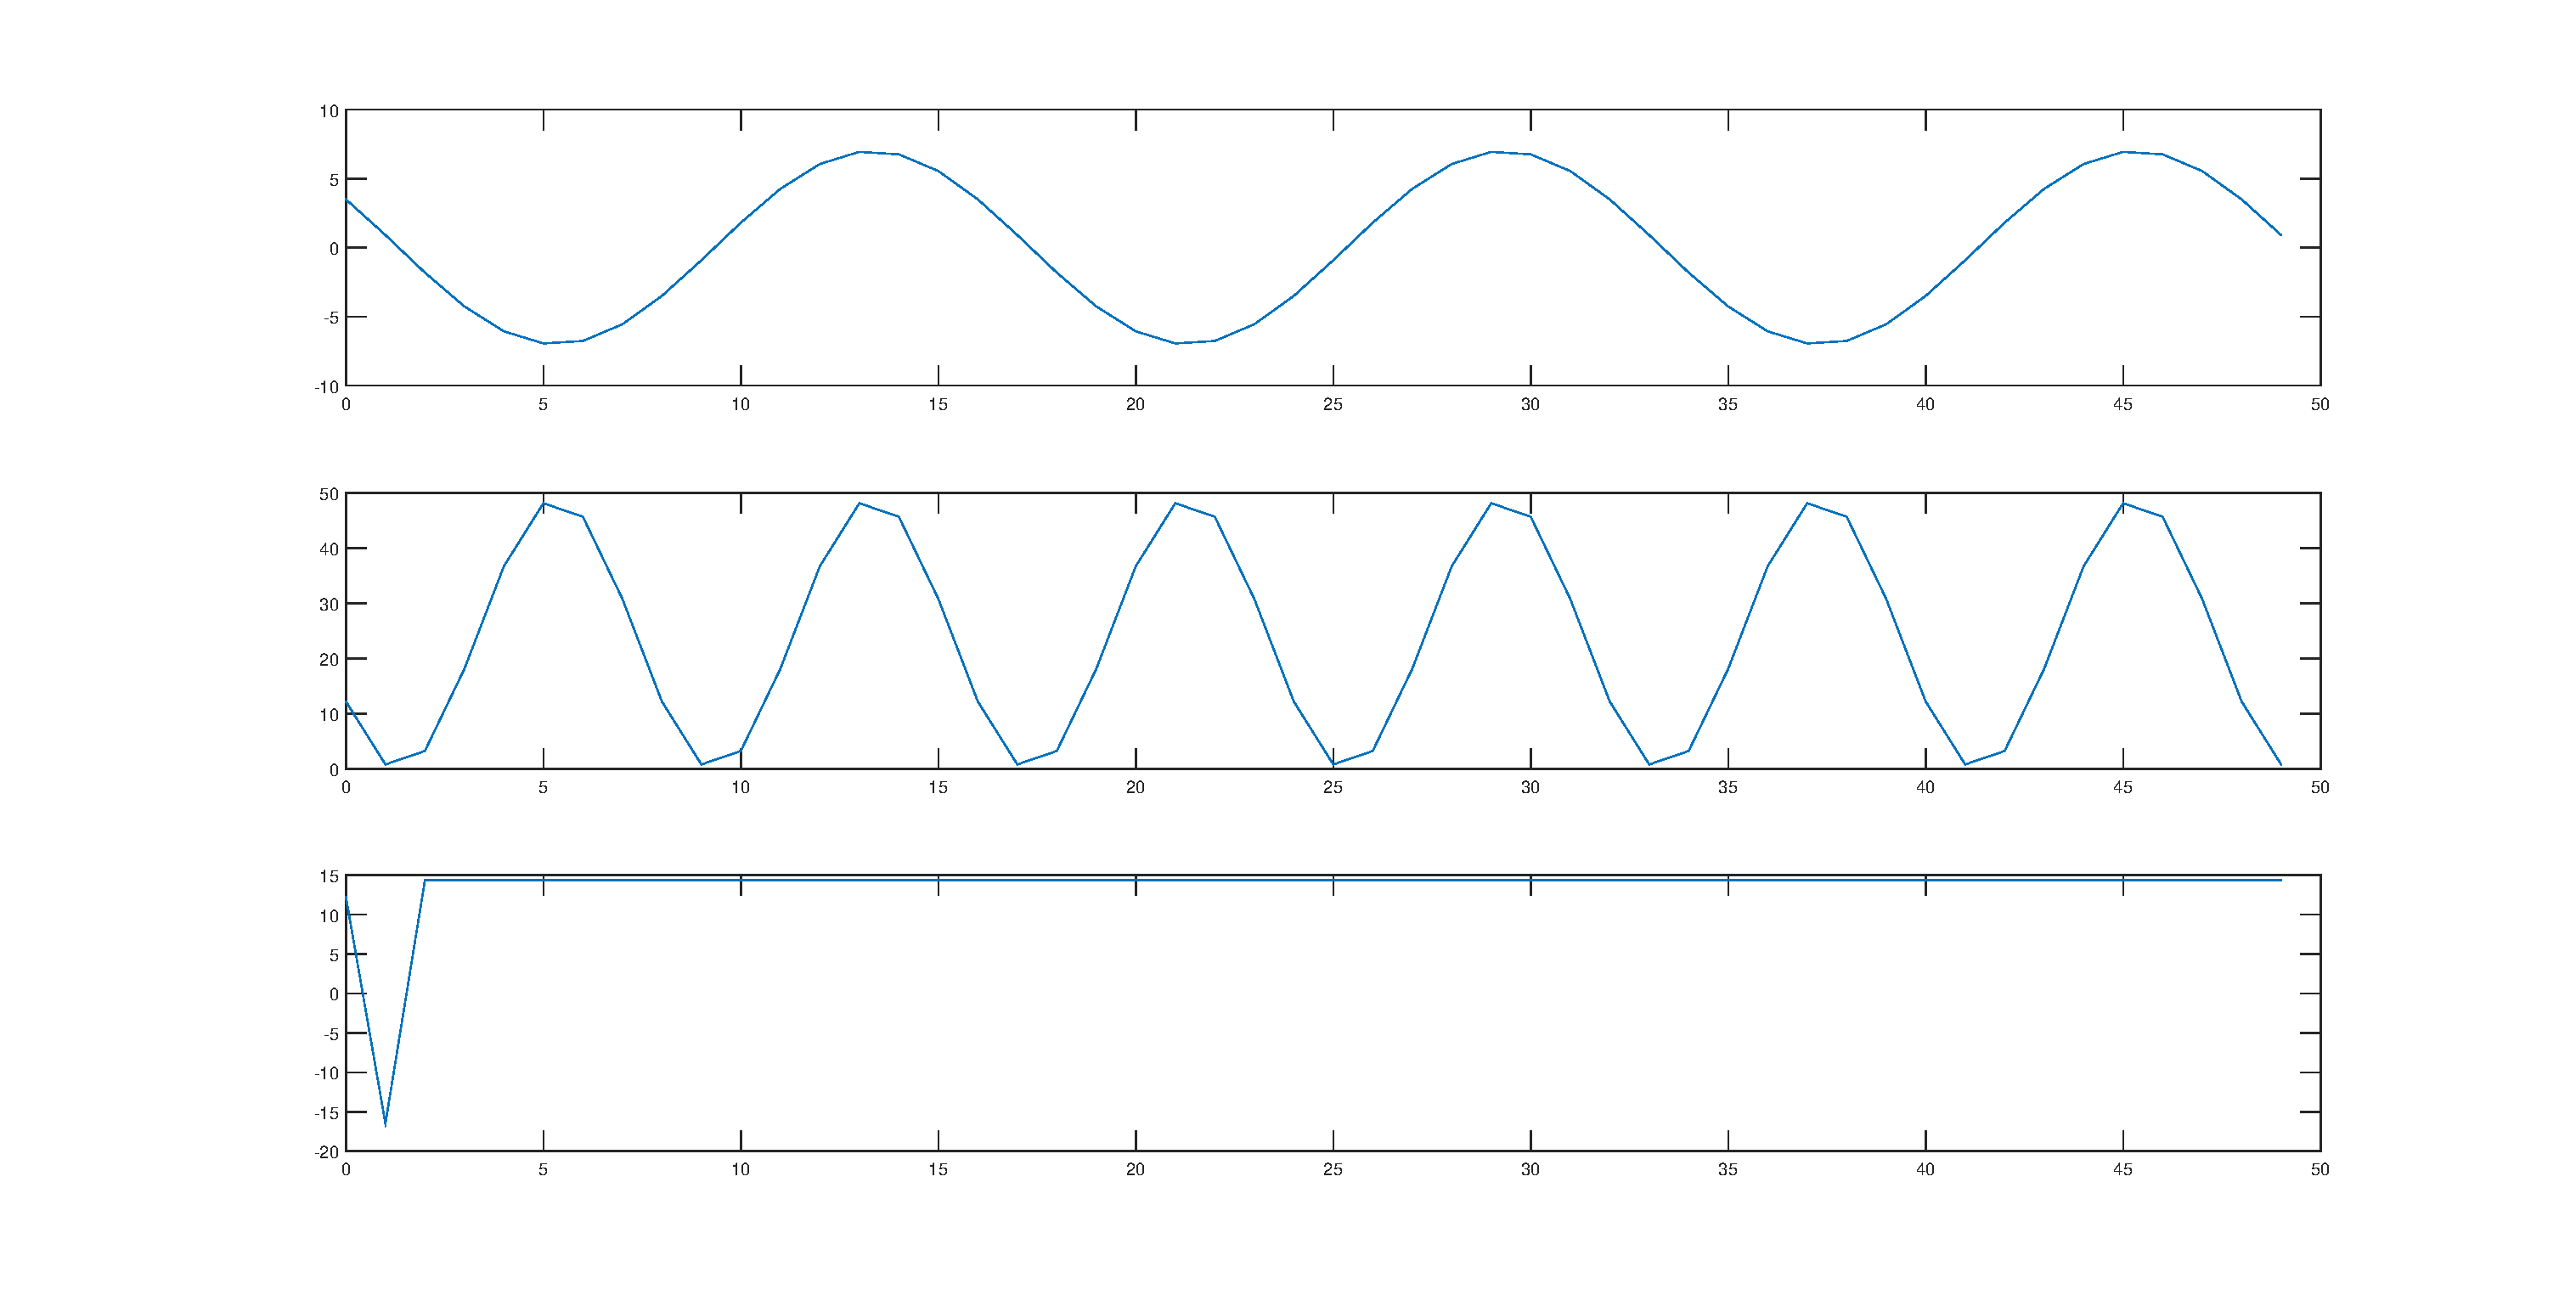
\includegraphics[scale=0.25]{fig11}
	\caption{Time series plot of the input signal, the squared signal and the final signal after the squared signal is passed through the first difference filter}
\end{figure}

\begin{figure}[H]
	\centering
	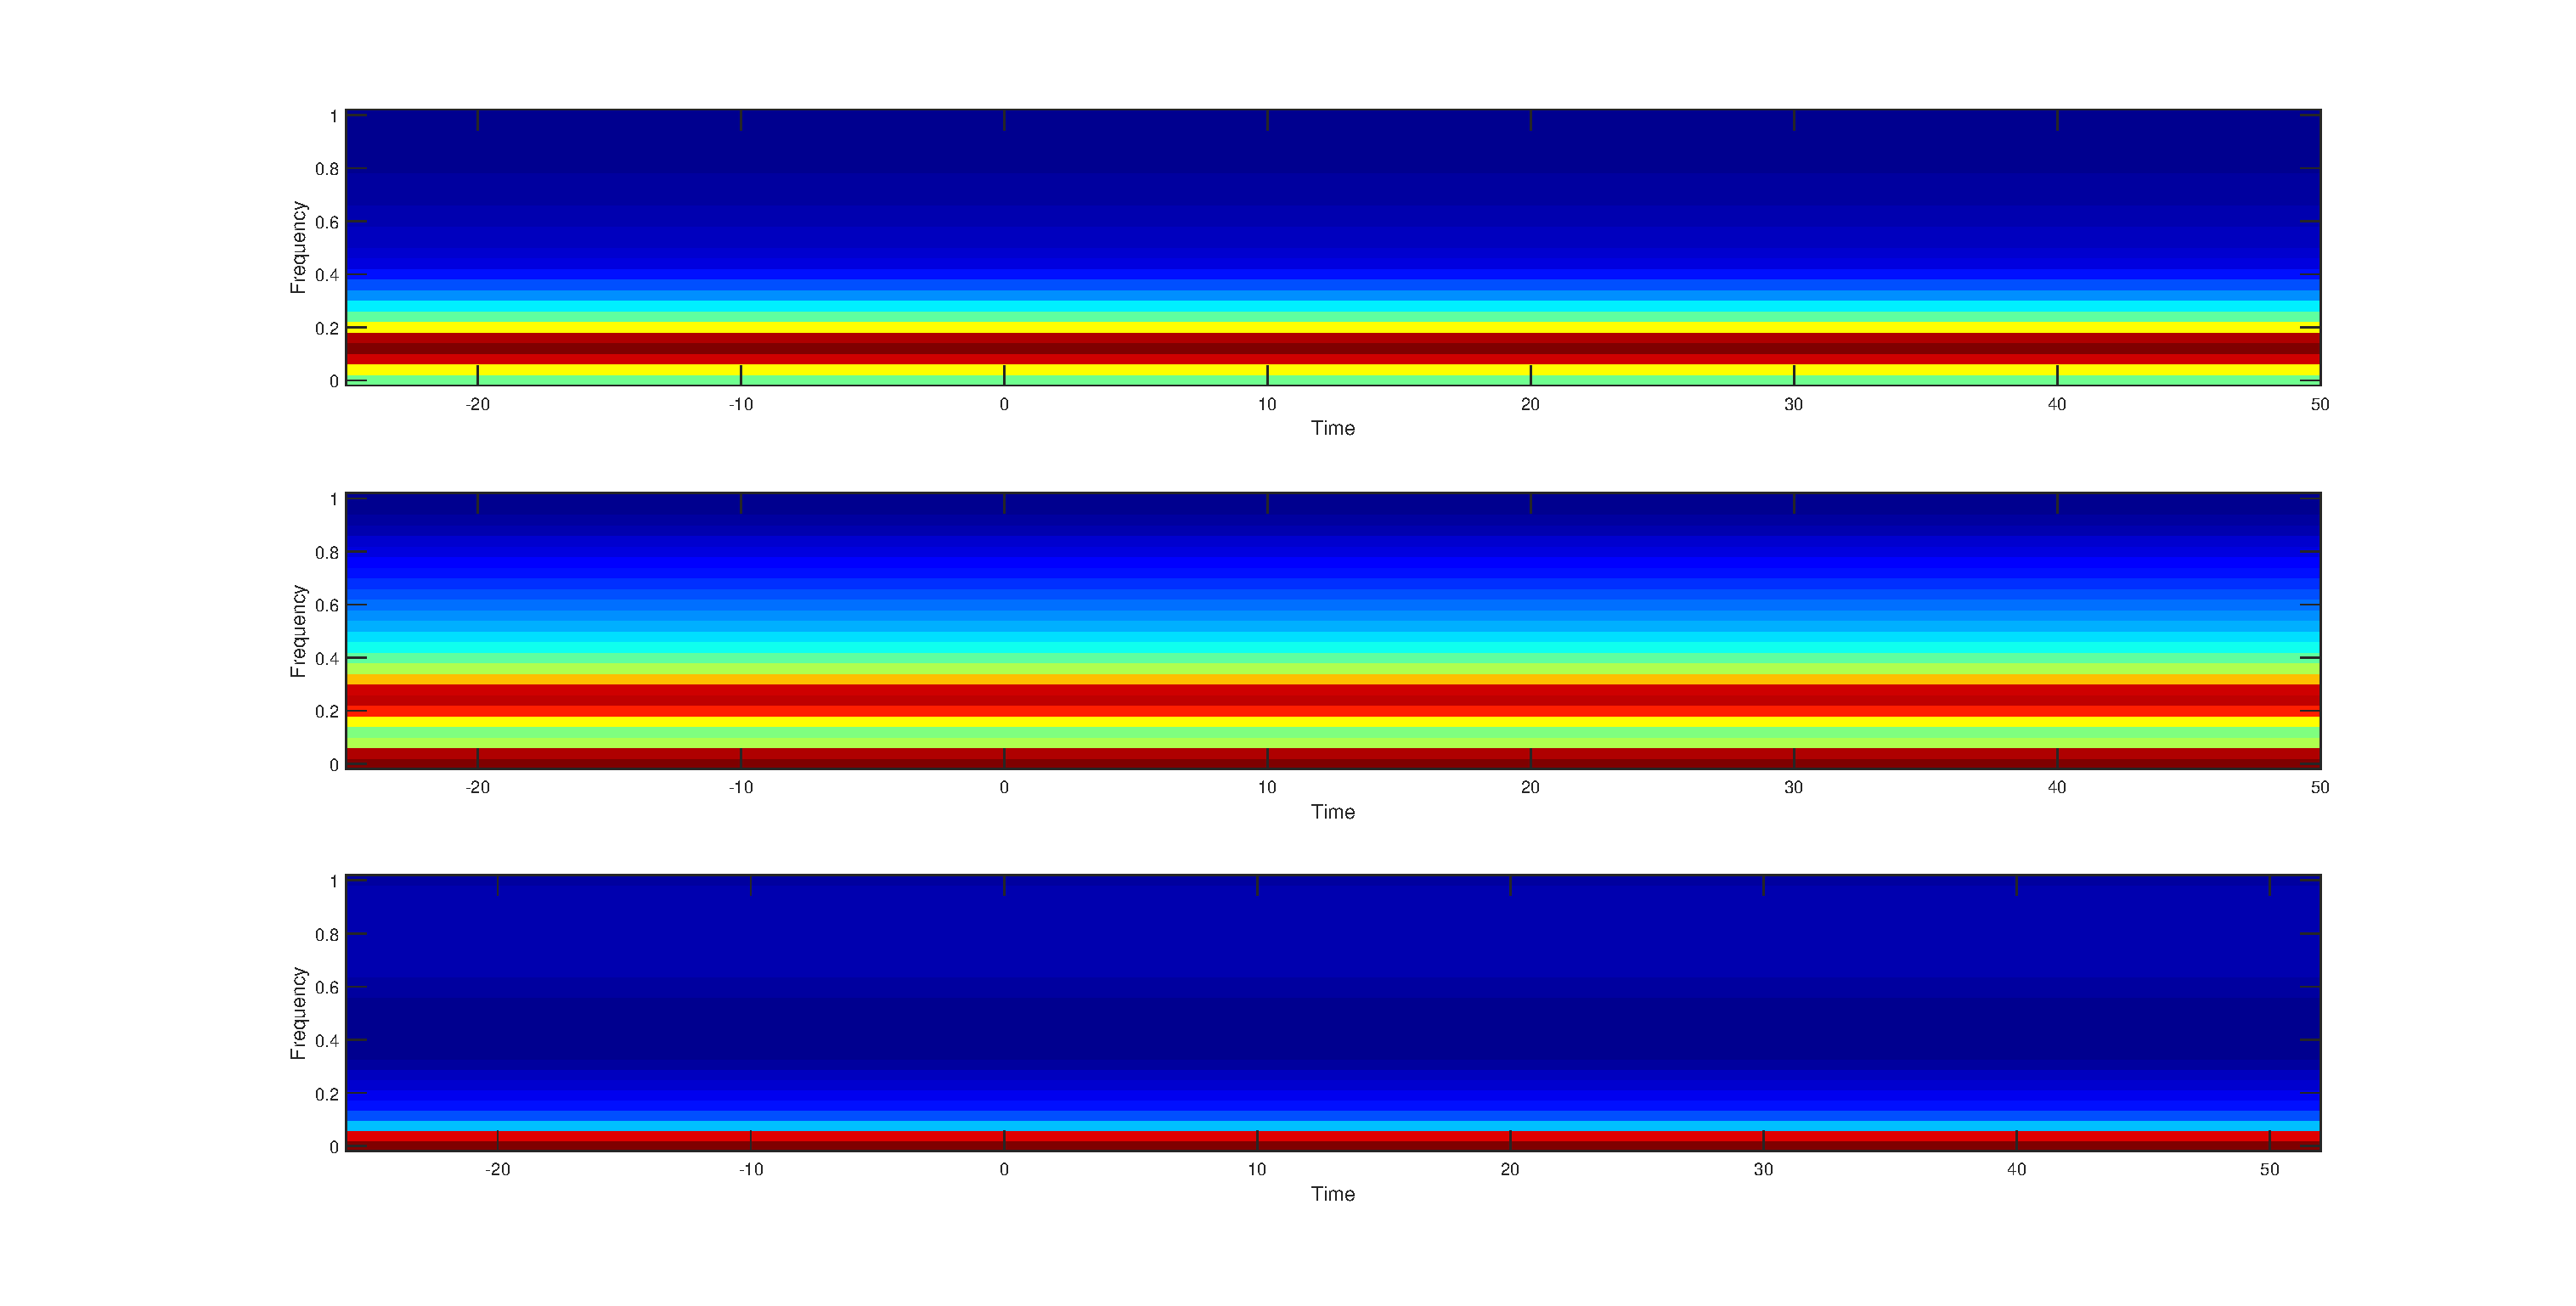
\includegraphics[scale=0.25]{fig12}
	\caption{A spectrogram of all three stages of signal}
\end{figure}

\end{document}